%%%% ijcai25.tex

\typeout{IJCAI--25 Instructions for Authors}

% These are the instructions for authors for IJCAI-25.

\documentclass{article}
\pdfpagewidth=8.5in
\pdfpageheight=11in

% The file ijcai25.sty is a copy from ijcai22.sty
% The file ijcai22.sty is NOT the same as previous years'
\usepackage{ijcai25}

% Use the postscript times font!
\usepackage{times}
\usepackage{soul}
\usepackage{url}
\usepackage[hidelinks]{hyperref}
\usepackage[utf8]{inputenc}
\usepackage[small]{caption}
\usepackage{graphicx}
\usepackage{amsmath}
\usepackage{amsthm}
\usepackage{booktabs}
\usepackage{algorithm}
\usepackage{algorithmic}
\usepackage[switch]{lineno}

% Added:
\usepackage{amssymb} % added
\allowdisplaybreaks 
\usepackage{tikz}
\usepackage{pgfplots}
\pgfplotsset{compat=1.18}
\usetikzlibrary{patterns,pgfplots.fillbetween}
\usepackage{subcaption} % For subfigures
\definecolor{darkgreen}{rgb}{0.0, 0.5, 0.0} % A dark green in RGB
\definecolor{darkred}{rgb}{0.65, 0.0, 0.0} % A dark red in RGB
\definecolor{darkblue}{rgb}{0.0, 0.0, 0.65} % A dark blue in RGB
\definecolor{darkyellow}{rgb}{0.75, 0.6, 0.0} % A dark yellow in RGB
\definecolor{custompurple}{RGB}{148, 103, 189} % Brown
\definecolor{darkorange}{RGB}{180, 120, 0} % Darker Orange

% Comment out this line in the camera-ready submission
% \linenumbers
\urlstyle{same}

% the following package is optional:
%\usepackage{latexsym}

% See https://www.overleaf.com/learn/latex/theorems_and_proofs
% for a nice explanation of how to define new theorems, but keep
% in mind that the amsthm package is already included in this
% template and that you must *not* alter the styling.
\newtheorem{example}{Example}
\newtheorem{theorem}{Theorem}

% Following comment is from ijcai97-submit.tex:
% The preparation of these files was supported by Schlumberger Palo Alto
% Research, AT\&T Bell Laboratories, and Morgan Kaufmann Publishers.
% Shirley Jowell, of Morgan Kaufmann Publishers, and Peter F.
% Patel-Schneider, of AT\&T Bell Laboratories collaborated on their
% preparation.

% These instructions can be modified and used in other conferences as long
% as credit to the authors and supporting agencies is retained, this notice
% is not changed, and further modification or reuse is not restricted.
% Neither Shirley Jowell nor Peter F. Patel-Schneider can be listed as
% contacts for providing assistance without their prior permission.

% To use for other conferences, change references to files and the
% conference appropriate and use other authors, contacts, publishers, and
% organizations.
% Also change the deadline and address for returning papers and the length and
% page charge instructions.
% Put where the files are available in the appropriate places.


% PDF Info Is REQUIRED.

% Please leave this \pdfinfo block untouched both for the submission and
% Camera Ready Copy. Do not include Title and Author information in the pdfinfo section
\pdfinfo{
/Title (Navigating Demand Uncertainty in Container Shipping: Deep Reinforcement Learning for Enabling Adaptive and Feasible Master Stowage Planning)
/Author (J. van Twiller, Y. Adulyasak, E. Delage, D. Grbic, R.M. Jensen)}

\title{Navigating Demand Uncertainty in Container Shipping: Deep Reinforcement Learning for Enabling Adaptive and Feasible Master Stowage Planning\footnote{This paper is currently under review for IJCAI 2025.}}

% Single author syntax
\author{
    Jaike van Twiller$^1$\and
    Yossiri Adulyasak$^2$\and
    Erick Delage$^2$\and
    Djordje Grbic$^1$\and
    Rune Møller Jensen$^1$ \\
    \affiliations
    $^1$ IT University of Copenhagen, Denmark \\
    $^2$ HEC Montréal, Canada \\
    \emails
    \{jaiv, djgr, rmj\}@itu.dk, \\
    \{yossiri.adulyasak, erick.delage\}@hec.ca
}


% \author{Anonymous submission}

% \author{
%     Author Name
%     \affiliations
%     Affiliation
%     \emails
%     email@example.com
% }

% % Multiple author syntax (remove the single-author syntax above and the \iffalse ... \fi here)
% \iffalse
% \author{
% First Author$^1$
% \and
% Second Author$^2$\and
% Third Author$^{2,3}$\And
% Fourth Author$^4$\\
% \affiliations
% $^1$First Affiliation\\
% $^2$Second Affiliation\\
% $^3$Third Affiliation\\
% $^4$Fourth Affiliation\\
% \emails
% \{first, second\}@example.com,
% third@other.example.com,
% fourth@example.com
% }
% \fi

\begin{document}

\maketitle

\begin{abstract}
Reinforcement learning (RL) has shown promise in solving various combinatorial optimization problems. However, conventional RL faces challenges when dealing with real-world constraints, especially when action space feasibility is explicit and dependent on the corresponding state or trajectory. In this work, we focus on using RL in container shipping, often considered the cornerstone of global trade, by dealing with the critical challenge of master stowage planning. The main objective is to maximize cargo revenue and minimize operational costs while navigating demand uncertainty and various complex operational constraints, namely vessel capacity and stability, which must be dynamically updated along the vessel's voyage. To address this problem, we implement a deep reinforcement learning framework with feasibility projection to solve the master stowage planning problem (MPP) under demand uncertainty. The experimental results show that our architecture efficiently finds adaptive, feasible solutions for this multi-stage stochastic optimization problem, outperforming traditional mixed-integer programming and RL with feasibility regularization. Our AI-driven decision-support policy enables adaptive and feasible planning under uncertainty, optimizing operational efficiency and capacity utilization while contributing to sustainable and resilient global supply chains.
\end{abstract}
\section{Introduction}
In recent years, machine learning (ML) for combinatorial optimization (CO) has gained much traction \cite{bengio_machine_2021}. Learning advanced planning policies yields promising results in solving CO problems in transportation and logistics. Such approaches can outperform existing solution methods in some well-known problems, such as vehicle routing \cite{kool_attention_2019,hottung_efficient_2022} or job shop scheduling \cite{kwon_pomo_2020}. Even though it is important to benchmark algorithms on traditional CO problems, a significant opportunity remains to address lesser-known yet critical planning challenges in supply chains. By addressing these challenges, we bridge the gap between theory and practice, enhancing the reliability and efficiency of worldwide supply chain operations.

Container shipping is a key component of the global supply chain, responsible for transporting 45\% of annual goods valued at \$8.1 trillion \cite{unctad_review_2021}. Due to its scale, it is often regarded as the cornerstone of worldwide trade and modern consumerism. However, this scale also has a significant environmental impact, with yearly CO2 emissions exceeding 200  million tonnes \cite{lloyds_list_shipping_2022}. Despite this, container vessels are considered an environmentally friendly mode of transportation, due to their relatively low emissions per cargo ton-mile \cite{jensen_container_2018}. Consequently, container shipping is recognized to play a crucial role in the global green transition \cite{european_commission_reducing_2023}. Within container shipping, there are several interdependent and complex planning tasks, such as berth allocation \cite{martin-iradi_multiport_2022}, pre-marshalling \cite{hottung_deep_2020}, quay crane scheduling \cite{herup_linear_2022}, and container vessel stowage planning \cite{van_twiller_literature_2024}. Due to decision-making under demand uncertainty and various combinatorial aspects - such as capacity limits, seaworthiness requirements, minimizing overstowage and maximizing revenue - stowage planning is particularly challenging. To mitigate this challenge, stowage planning is often decomposed into the master planning problem (MPP), which involves the assignment of cargo to clusters of slots, and the slot planning problem (SPP), which allocates containers to individual slots \cite{pacino_fast_2011}. However, these subproblems in representative form, particularly the MPP, remain non-trivial and difficult to solve especially in the presence of uncertainty \cite{van_twiller_literature_2024}. 

In addition to its complexity, stowage planning faces public data scarcity and relies heavily on human planners supported by limited decision support systems \cite{jensen_container_2018}. Planners should maximize capacity utilization while managing demand uncertainty by accounting for multiple future scenarios. However, evaluating such scenarios is computationally intractable, due to the problem's complexity and dynamic nature. These limitations highlight the need for efficient, adaptive, and feasible decision-support systems, offering an opportunity for AI-driven solution methods to enhance the resilience and sustainability of the global supply chain.

This paper presents a deep reinforcement learning (DRL) approach with feasibility projection to construct adaptive and feasible solutions, providing a decision-support policy for the MPP under demand uncertainty.

Our main contributions are as follows:
\begin{itemize}
    \item \textbf{Master Stowage Planning Environment:} We develop a novel Markov decision process (MDP) for master stowage planning under demand uncertainty, incorporating realistic problem-specific constraints. To address data scarcity, we release the environment as an open-source implementation\footnote{\url{https://github.com/OptimalPursuit/navigating_uncertainty_in_mpp}}.    %\footnote{\url{https://anonymous.4open.science/r/navigating_uncertainty_in_mpp-45CE/}}. \footnote{\url{https://github.com/OptimalPursuit/DRL_4_master_planning}}
    \item \textbf{Feasibility Projection:} We incorporate differentiable projection layers, including weighted scaling, policy clipping, and violation projection, to enforce inequality constraint satisfaction in DRL frameworks.
    \item \textbf{Efficient and Adaptive Solutions:} Our experiments demonstrate that our policy efficiently generates adaptive and feasible solutions under demand uncertainty, significantly outperforming well-known DRL methods and a multi-stage stochastic MIP model.
    \item \textbf{Decision Support for Stowage Planning:} Our decision-support policy transcends deterministic models, enabling dynamic and uncertainty-informed planning in a critical part of the global supply chain.   
\end{itemize}

\section{Domain Preliminaries} \label{sec:domain}
We present the preliminaries of the stowage planning domain to provide the planning context. We refer to \cite{jensen_container_2018} for a comprehensive review.

\textbf{Voyages.} Liner shipping companies utilize fleets of container vessels that operate on fixed schedules along a closed-loop course, similar to a maritime bus service that carries goods between ports. The complete journey covering all ports is called a voyage, typically starting in regions with a supply surplus (e.g., Asia) and navigating towards high-demand discharge areas (e.g., Europe), often voyages cover more than ten ports. A voyage can be described as a directed path graph $G_P = (P, E_P)$ with nodes being $P = \{1,2,\dots, N_P\}$, and edges being legs between ports $E_P = \{ (p, p\!+\!1) \mid p \in \{1, 2, \dots, N_P\!-\!1\} \}$ with $N_P$ being the last port. We also define sub-voyages by set ${P}_\text{start}^\text{end} = \{p \in {P}\!\mid\! \text{start}\leq p \leq \text{end}\}$. 

Containers have a port of load (\textit{pol}) and a port of discharge (\textit{pod}), also named transports or origin-destination pairs. Consider $\textit{pol} \in {P}_1^{N_P-1}$ and $\textit{pod} \in {P}_{2}^{N_P}$ with $P^2 = P \times P$, which can be represented by transport $\textit{tr} = (\textit{pol},\textit{pod})$. We can define a set of transports $\textit{TR}=\{(i,j) \in {P}^2\!\mid\! i<j\}$. 

\textbf{Container Cargo.} Containers vary in dimensions and types, but we focus on the most common and impactful characteristics: lengths (20 ft, 40 ft), weight classes (light, medium, heavy), and customer types (long-term, spot market). Container revenue is driven by customer contract types, where $\textit{rev}$ is the revenue depending on cargo type and transport. Long-term contracts provide lower revenue but ensure high, stable volumes, whereas spot market contracts yield higher revenue with lower, more volatile volumes. Long-term contracts are prioritized over spot contracts. However, the lack of no-show fees creates inherent uncertainty in container demand, which becomes more predictable as the arrival date approaches. Consequently, planners must dynamically allocate cargo to vessels during the voyage while managing uncertainty. Containers are often grouped into cargo classes by characteristics, such as ${K} = \{20\textit{ft}, 40\textit{ft}\} \times \{\textit{Light}, \textit{Medium}, \textit{Heavy}\} \times \{\textit{Spot},\textit{Long}\}.$

\textbf{Vessel Layout.} Figure \ref{fig:vessel1} shows the cellular layout of container vessels with standardized coordinates of \textit{(bay, row, tier)}. It is divided into bays (02-38) ranging from the front (e.g., bay 02) to the rear (e.g., bay 38), also named from fore to aft. Bays are defined by an ordered set ${B} = \{1,2,\dots,N_B\}$, ranging from fore to aft with $N_B$ being the last bay. Each bay contains stacks of cells, whereas cells contain two slots that can hold two 20-foot containers or one 40-foot container. Bays are horizontally separated by hatch covers into above and below deck sections, introducing the set of decks ${D} = \{d^\textit{above}, d^\textit{below}\}$. It is worth noting that hatch covers introduce complexity since below-deck cargo can only be discharged if the above-deck cargo is cleared.

\begin{figure}[t]
\includegraphics[scale=0.28]{figures/VesselSideTop.pdf}
\caption{The side and top view of a container vessel.}
\label{fig:vessel1}
\end{figure}

\textbf{Utilization.} Vessel utilization  \( u_p \in \mathbb{Z}^{|B| \times |D| \times |K| \times |\textit{TR}|} \) represents the cargo placement across bays $B$, decks $D$, cargo types $K$, and transports $\textit{TR}$. Load operations are defined by $u^+_p \in \mathbb{Z}_{>0}^{|B| \times |D| \times |K| \times |\textit{TR}|}$, whereas discharging is denoted by $u^-_p \in \mathbb{Z}_{>0}^{|B| \times |D| \times |K| \times |\textit{TR}|}$. The utilization at port $p$ is defined as $u_p = u_{p-1} + u^+_p - u^-_p \; \forall p \in {P}$, where $u_0$ is the vessel's arrival condition at the first port. We also define the vessel's pre-loading utilization $u'_p = u_{p-1} - u^-_p$.

\textbf{Objectives and Global Constraints.} The MPP aims to create a capacity management plan for each general location (indexed by bay and deck) while adhering to global constraints, as outlined below. The MPP maximizes revenue by optimizing capacity for high-value cargo and minimizes costs through improved operational efficiency. The SPP then assigns containers to slots within the general locations while considering local constraints. Due to frequent re-planning as new information arises, algorithmic runtimes over 10 minutes are impractical for real-world operations \cite{pacino_fast_2011}.

Vessels have different types of capacity related to TEUs, height, weight and special cargo. The amount to which this can be utilized depends on the arrival condition of vessels and uncertain cargo demand. It is therefore non-trivial to ensure optimal utilization of vessel capacities. The key efficiency objectives are minimizing overstowage, an NP-hard task \cite{tierney_complexity_2014}, and minimizing the quay crane makespan. Overstowage occurs when containers stacked on top block access to those below in need of discharging, requiring additional crane operations to remove and reload the obstructing containers, thereby increasing the workload. In addition, the crane makespan considerably impacts the port stay duration, while ports set makespan targets and overruns incur costs. It is thus beneficial to minimize the makespan by maximizing the average use of parallel cranes, thereby minimizing idle time. 

Furthermore and most importantly, vessels must adhere to safety requirements to ensure seaworthiness, which is heavily influenced by weight distribution. Before introducing the constraints, we first clarify that $\otimes$ represents the outer product and $\odot$ denotes the element-wise Hadamard product, with broadcasting applied when shapes are compatible. The longitudinal (\textit{lcg}) and vertical centres of gravity (\textit{vcg}), which are associated with trim and metacentric height, of the load $u_p$ prior to leaving port $p$ must remain within specified bounds (\( \underline{\textit{lcg}}, \overline{\textit{lcg}} \in \mathbb{R}_{>0} \)), as shown in Constraints \eqref{for:lcg} and \eqref{for:vcg}. To compute the stability, we define the longitudinal moment \(\textit{lm} = \textit{ld} \otimes w\) and vertical moment \(\textit{vm} = \textit{vd} \otimes w\), where \( w \in \mathbb{R}^{|K|\times|\textit{TR}|}_{>0} \) represents container weights, and \( \textit{ld}, \textit{vd} \in \mathbb{R}^{|B| \times |D|} \) denote the longitudinal and vertical distances of positions from the vessel's centre of gravity. 
\begin{align}
\underline{\textit{lcg}} \leq \frac{\mathbf{1}^\top \big( \textit{lm} \odot u_p \big)}{\mathbf{1}^\top \big( w \odot u_p \big)} \leq \overline{\textit{lcg}}, \qquad \forall p \in P \label{for:lcg} \\
\underline{\textit{vcg}} \leq \frac{\mathbf{1}^\top \big( \textit{vm} \odot u_p \big)}{\mathbf{1}^\top \big( w \odot u_p \big)} \leq \overline{\textit{vcg}}, \qquad \forall p \in P \label{for:vcg}
\end{align}

In conclusion, the scale and complexity of the problem pose significant challenges. As a result, most models focus on subsets of realistic constraints to remain tractable, often requiring human intervention to ensure practical usability.

\section{Related Work}
This section positions our work in the literature on stowage planning, stochastic programming and ML in optimization.  

\textbf{Stowage Planning.} To address the complexity of stowage planning, various solution approaches have been applied to different problem formulations, including exact methods \cite{roberti_decomposition_2018}, linearly relaxed MIP \cite{pacino_fast_2011}, matheuristics \cite{parreno-torres_solving_2021}, population-based metaheuristics \cite{chang_solving_2022}, neighbourhood-based metaheuristics \cite{pacino_crane_2018}, hybrid frameworks \cite{bilican_mathematical_2020}. 
Despite these techniques, a recent survey highlights that scalable solutions for representative stowage and MPP problems remain unsolved \cite{van_twiller_literature_2024}. Research has largely focused on deterministic problems, overlooking real-world needs for profit maximization in the face of demand uncertainty. 

\textbf{Stochastic Programming.} Decision-making under uncertainty is traditionally approached through stochastic programming, where uncertainty is explicitly represented as a set of discrete scenarios evolving over multiple stages in time, approximating the underlying probability distribution \cite{birge_introduction_2011}. This process results in a scenario tree, whose computational complexity grows exponentially as $\mathcal{O}(b^T)$, where $b$ is the branching factor and $T$ is the number of stages. Hence, multi-stage problems with $T > 2$ and a reasonably large $b$ are often intractable. Common techniques to overcome this complication are scenario reduction to reduce problem size \cite{watanabe_scenario_2009}, decomposition techniques like Benders decomposition or Lagrangian relaxation to divide the problem \cite{rahmaniani_benders_2017}, progressive hedging to enforce non-anticipativity iteratively \cite{boland_combining_2018}, or approximation methods, such as stochastic dual dynamic programming \cite{shapiro_analysis_2011} and sample average approximation \cite{chen_sample_2022}, to enhance tractability while preserving solution quality.

\textbf{Learning with Hard Constraints.} In learning solution heuristics, a challenge arises to ensure feasibility in complex action spaces. This challenge is exacerbated when dealing with the dependence on state variables to define the feasible region. Several deep learning approaches have dealt with learning constraints by backpropagation through (in)equality completion \cite{donti_dc3_2021}, or differentiable projection layers, such as mapping interior points to boundaries \cite{li_learning_2023},  convex programming layers \cite{agrawal_differentiable_2019}, or problem-specific repair layers \cite{chen_end--end_2024}. Moreover, safe reinforcement learning has dealt with constraints by, e.g., constrained MDPs with a primal-dual approach \cite{ding_natural_2020}, soft barriers function \cite{wang_enforcing_2023}, and safety shields \cite{alshiekh_safe_2018}.

\section{Markov Decision Processes}
We present a formal MDP and a decomposed MDP to solve using DRL approaches. Technical details about both MDPs are provided in Appendix \ref{app:MDP}.

\subsection{Formal MDP}
Let ${\mathcal{M}} = ({S}, {X}, \mathcal{T}, {\mathcal{R}}, {P}^{N_P-1}_1, \gamma)$ define an episodic discounted MDP representing the MPP, where ${S}$ is a set of states, ${X}$ is a set of actions, $ \mathcal{T}: {S} \times {X} \rightarrow \Delta({S})$ is the transition function, $ {\mathcal{R}}: {S} \times {X} \times {P}^{N_P-1}_1 \rightarrow \mathbb{R}$ is the reward function, ${P}^{N_P-1}_1$ is the finite horizon of load ports with $N_P-1$ being the last port, and $\gamma \in (0,1]$ is the discounting factor.

\textbf{State.} The state is given by ${s}_p \in {S}$, defined as ${s}_p = (u_p, q_p, \zeta)$. This includes vessel utilization $u_p \in  \mathbb{R}_{\geq0}^{n_u}$ and realized demand $q_p \in  \mathbb{R}_{\geq0}^{n_q}$, where $n_u = |B|\times|D|\times|K|\times|\textit{TR}|$, $n_c = |B|\times|D|$ and $n_q = |K|\times|\textit{TR}|$ are the shapes of utilization, location and demand, respectively. 

Additionally, environment parameters $\zeta$ contain the expected value $\mu \in \mathbb{R}^{n_q}_{\geq 0}$ and standard deviation $\sigma \in \mathbb{R}^{n_q}_{> 0}$ of demand, load ports $i$, discharge ports $j$ and cargo types $k$ as $(i,j,k) \in \textit{TR} \times K$, TEU per container $\textit{teu} \in \{1,2\}^{n_q}$, cargo weight $w \in \mathbb{R}^{n_q}_{>0} $,  cargo revenue $\textit{rev} \in \mathbb{R}^{n_q}_{>0}$.

The initial state $s_0  = (u_0, q_0,\zeta)$ consists of an empty vessel $u_0 = \mathbf{0}^{n_u}$,  realized demand $q_0$ at initial port, and $\zeta$ is initialized randomly for each episode.

\textbf{Action.} An action $ {x}_p \in {X} $ assigns a real number of containers to utilization $u_p$, where ${x}_p \in \mathbb{R}_{>0}^{n_u}$ and thus similar to $u^+_p$. Each action $ {x}_p $ is subject to a feasible region, defined by polyhedron $ \textit{PH}({s}_p) = \{{x}_p \in \mathbb{R}^{n_u}_{>0} : A({s}_p) {x}_p \leq b({s}_p)\} $. Here, $ A({s}_p) \in \mathbb{R}^{m_u \times {n_u}} $ is the constraint matrix, $ b({s}_p) \in \mathbb{R}^{m_u} $ is the bound vector, and $m_u$ is the number of constraints. 

Previous work demonstrated that linearly relaxed MPPs outperform exact MPPs, as the subsequent SPP effectively discretizes the solution \cite{pacino_fast_2011}. Accordingly, we can adopt real-valued actions instead of integer-valued actions. Given a traditional MPP formulation with utilization \( u_p \) \cite{van_twiller_efficient_2024}, we define constraints of \( \textit{PH}({s}_p) \)  in terms of actions \( {x}_p \) and pre-loading utilization \( u'_p \). 
\begin{align}
\quad {x}_p^\top \mathbf{1}_{n_c} & \leq \; q_p  \label{for:fr_demand}\\
\quad  {x}_p \textit{teu} & \leq \; c - u'_p \textit{teu} \label{for:fr_capacity}\\
\text{-}\mathbf{1}^\top \! \big((\textit{lm}\!-\!\underline{\textit{lcg}} w)\!\odot\!{x}_p \big) & \leq \! \text{-}\mathbf{1}^\top\! \big( (\underline{\textit{lcg}} w\!-\!\textit{lm})\!\odot\!u'_p \big) \label{for:fr_lcg_lb} \\
\;\mathbf{1}^\top \! \big( (\textit{lm}\!-\!\overline{\textit{lcg}} w)\!\odot\!{x}_p \big) & \leq \! \; \mathbf{1}^\top\!\big( (\overline{\textit{lcg}} w\!-\!\textit{lm})\!\odot\!u'_p \big) \label{for:fr_lcg_ub} \\
\text{-}\mathbf{1}^\top \! \big((\textit{vm}\!-\!\underline{\textit{vcg}} w)\!\odot\!{x}_p \big) & \leq \! \text{-}\mathbf{1}^\top\!\big( (\underline{\textit{vcg}} w\!-\!\textit{vm})\!\odot\!u'_p \big) \label{for:fr_vcg_lb} \\
\;\mathbf{1}^\top \! \big((\textit{vm}\!-\!\overline{\textit{vcg}} w)\!\odot\!{x}_p \big) & \leq \! \; \mathbf{1}^\top\!  \big( (\overline{\textit{vcg}} w\!-\!\textit{vm})\!\odot\!u'_p \big) \label{for:fr_vcg_ub}
\end{align}

Constraint \eqref{for:fr_demand} limits load \( {x}_p \) to the available demand \( q_p \), while Constraint \eqref{for:fr_capacity} ensures \( {x}_p \) does not exceed the residual TEU capacity. Constraints \eqref{for:fr_lcg_lb}–\eqref{for:fr_lcg_ub} enforce lcg limits, while Constraints\eqref{for:fr_vcg_lb}–\eqref{for:fr_vcg_ub} impose similar bounds on the vcg. These stability bounds are derived from Constraints \eqref{for:lcg} and \eqref{for:vcg}.

\textbf{Transition.} We use a stochastic transition function \( \mathcal{T}({s}_{p+1} | {s}_p, {x}_p) \in \Delta({S}) \). Within an episode, the transition consists of multiple components:
\begin{itemize}
    \item Upon port arrival, port demand \( q_p \) is revealed.
    \item Subsequently, onboard cargo is discharged \( u_{p+1} = u_p \odot (1 - \mathbf{e}_p^-) \), where \( \mathbf{e}_p^- \in \{0, 1\}^{n_q} \) is a binary mask indicating the cargo type and transport to nullify in \( u_p \).
    \item Finally, cargo is loaded onboard \( u_{p+1} = u_p + {x}_p\). Action ${x}_p$ is based on the current utilization $u_p$ and revealed demand $q_p$ of port $p$. Future port demand stays unknown.
\end{itemize}

\textbf{Reward.}  Equation \eqref{for:reward} defines our deterministic reward function, computing profit as the difference between revenue and costs. Revenue is computed as the sum of \( x_p \) corresponding to elements of \( q_p \). Since revenue cannot be obtained from containers exceeding demand, the summation of \( x_p \) is restricted to the elements within \( q_p \).  While costs are computed via the state-dependent auxiliary variables hatch overstows \( \textit{ho}({s}_p,p) \in  \mathbb{R}^{|B|}_{>0} \) and excess crane moves \( \textit{cm}({s}_p,p) \in \mathbb{R}^{|B|-1}_{>0}  \). These costs are weighted by \( \textit{ct}^\textit{ho} \in \mathbb{R}_{>0} \) and \( \textit{ct}^\textit{cm} \in \mathbb{R}_{>0}\), respectively.
\begin{align} \label{for:reward}
\mathcal{R}(s, x, p) = & \; \textit{rev} \min\big(x^\top \mathbf{1}_{n_c}, q \big)\nonumber \\ 
& - \textit{ct}^\textit{ho} \mathbf{1}^\top \textit{ho}(s, p) + \textit{ct}^\textit{cm} \mathbf{1}^\top \textit{cm}(s, p).
\end{align}

\subsection{Decomposed MDP}
The formal MDP defines an effective action space of size $|{X}| \propto |B| \cdot |D| \cdot |K| \cdot |P|$, where each action ${x}_p$ determines how cargo types and transport options are placed on the vessel per port. However, this action space is large, which can hinder learning efficiency \cite{kanervisto_action_2020}. 

To address this, we decompose the formal MDP into granular, sequential steps based on an index $(i,j,k) \; \forall (i,j) \in \textit{TR}, k \in K$. Instead of placing all transport and cargo types simultaneously, we take a decomposed action for all transports $(p,j)$ and cargo types $k$ at port $p$, then departing to a new port. This reduces the action space to $|X| = |B| \cdot |D|$, while unfolding transports and cargo types over an extended time horizon $t \in H = \{0,1,\dots,T_\textit{seq}\}$ with 
\(T_\textit{seq} = |K| \cdot |\textit{TR}|.\)

\textbf{State.} The state $s_t = (u_t, q_t, \zeta)$ depends on time step $t$, where $u_t \in \mathbb{R}^{n_u}_{\geq 0}$ is vessel utilization, and $q_t \in \mathbb{R}^{n_q}_{\geq 0}$ is realized demand. The environment parameter \( \zeta \) remains unchanged. Given the time $t$, however, we can extract relevant parameters from \( \zeta \), such as \( (\textit{pol}_t, \textit{pol}_t, k_t), \textit{rev}^{(\textit{pol}_t, \textit{pod}_t, k_t)} \). 

\textbf{Action.} Action $x_t \in \mathbb{R}^{n_c}_{\geq0}$ assigns real number of containers to utilization $u_t$ for step $t$. Each action is subject to $\textit{PH}(s_t) =  \{x_t \in \mathbb{R}^{n_c}_{>0} : A(s_t) x_t \leq b(s_t)\} $. Here, $ A(s_t) \in \mathbb{R}^{m_c \times {n_c}} $ is the constraint matrix, $ b(s_t) \in \mathbb{R}^{m_c} $ is the bound vector, and $m_c$ is the number of constraints. It is also worth noting that Constraints \eqref{for:fr_demand}-\eqref{for:fr_vcg_ub} are reformulated to fit feasible region $\textit{PH}(s_t)$.

\textbf{Transition.} At each time step \( t \), the transition includes loading, where \( x_t \) is added to \( u_t \). However, discharging and demand realization occur only when arriving at a new port, indicated by \( t \in T_{\text{new port}} \).

\textbf{Reward.} The revenue at step \( t \) is computed as \( \textit{rev}(\textit{pol}_t, \textit{pod}_t, k_t) \min(\mathbf{1}^\top x_t, q_t^{(\textit{pol}_t, \textit{pod}_t, k_t)}). \) However, costs depend on knowing all loading operations at port $p$, which is aggregated in utilization $u_t$ at the last step of the port \( t \in T_{\text{leave port}} \). As a result, the cost signal is sparse, being evaluated only once per port $p$, rather than at each step.

\section{Proposed Architecture}
Our approach consists of several components: an encoder-decoder model parameterized by $\theta$, an actor-critic DRL method, and a feasibility projection layer. The encoder-decoder model shown in Figure~\ref{fig:drl_architecture} employs a look-ahead policy \( \pi_{\theta}(x|s_t) \) conditioned on state \( s_t \) and parameterized by mean \( \mu_\theta(s_t) \) and standard deviation \( \sigma_\theta(s_t) \). By training in the decomposed MDP and optionally projecting the policy, we iteratively generate actions $x_t$ to construct solutions.

\begin{figure}[h!]
    \centering
    \includegraphics[width=\linewidth]{figures/DRL_Architecture.pdf}
    \caption{Deep Reinforcement Learning Architecture with Feasibility Projection for Actor-Critic Methods}
    \label{fig:drl_architecture}
\end{figure}

\subsection{Encoder-Decoder Model}
Figure \ref{fig:encoder_decoder_models} presents our encoder-decoder model, based on that of \cite{kool_attention_2019}, with modifications highlighted below.

\begin{figure}[t!]
    \centering
    \includegraphics[width=0.85\linewidth]{figures/Actor_Critic_Model.pdf}
    \caption{Layers of the encoder and the actor-critic decoder.}
    \label{fig:encoder_decoder_models}
\end{figure}

\textbf{Cargo Embedding.} The cargo embedding \( e^\text{cargo}(\zeta) \) parameterized by \( \theta_\textit{cr} \) maps cargo-related episode information in $\zeta$ into a feature representation for the encoder. To enhance positional awareness, we subsequently apply sinusoidal positional encoding \cite{vaswani_attention_2017}.

\textbf{Encoding Layers.} An attention encoder $f(e^\text{cargo}(\zeta))$ parameterized by ${\theta_\textit{enc}}$  maps embedding $e^\text{cargo}(\zeta)$ to latent variable $z$ using multi-head attention (MHA) to identify revalant features dynamically \cite{vaswani_attention_2017}. Then, we use a feed-forward network (FFN) with ReLU activation, layer normalization, residual connections, and dropout. 

\textbf{Context Embedding.} The context embedding $e^\text{cont}(u_t, z)$, parameterized by ${\theta_\textit{co}}$, focuses on time $t$, extracting time-specific features from the utilization $u_t$ and latent variable $z$. These features provide the MHA query with a representation of the vessel’s current condition, enabling the policy to make decisions based on the present context.

\textbf{Dynamic Embedding.} The dynamic embedding \(e^\text{dynam}(q_t, z) \), parameterized by ${\theta_\textit{dn}}$, extracts features from demand $q_t$ in all steps of horizon $H$, capturing patterns across the entire episode. It combines real demand and latent information to produce keys and values for the MHA layer. As such, it accounts for global temporal trends, allowing it to anticipate future conditions and make long-term decisions.

\textbf{Actor Layers.} As proposed in \cite{kool_attention_2019}, our actor decoder $g(e^\text{cont}(u_t, z), e^\text{dynam}(q_t, z))$ is an attention model parameterized by $\theta_\textit{act}$. However, our actor takes input from the context and dynamic embedding. An MHA layer with a forward-looking mask bases decisions on steps ${t, t+1, \dots, T_\textit{seq}}$ to anticipate future events. Subsequently, an FFN extracts features, after which a pointer mechanism performs a soft selection of relevant steps using key-value inputs \cite{vinyals_pointer_2015}. A softplus activation outputs positive logits $({\mu}_\theta(s_t), {\sigma}_\theta(s_t))$.

\textbf{Critic Layers.} Our critic model $V(s_t,z)$, parameterized by $\theta_\textit{cri}$, estimates the value of state $s_t$ and latent variable $z$ through an FFN outputting $V_{\theta_\textit{cri}}(s_t, z) \in \mathbb{R}$.

\textbf{Action Policy.} The actor logits parameterize a stochastic policy $\pi_{\theta}(x|s_t) = \mathcal{N}(({\mu}_\theta(s_t), {\sigma}_\theta(s_t))$, which allows action sampling $x_t \sim \pi_{\theta}(x|s_t)$ to construct solutions. 

\subsection{Feasibility Regularization in Actor-Critic Loss}  
Standard actor-critic methods can efficiently and stably learn policies that require implicit feasibility in the action space \cite{schulman_proximal_2017,haarnoja_soft_2018}, while explicit constraints are often integrated by feasibility regularization (FR) in the actor loss \cite{ding_natural_2020,calvo-fullana_state_2021}. Equation \eqref{for:feas_loss} defines a composite loss that combines the actor loss $\mathcal{L}_{\text{actor}}(\theta)$ with a soft regularization term $\mathcal{L}_{\text{feas}}(\theta)$. FR is defined in Equation \eqref{for:feas_loss}, where $\lambda_f$ controls the regularization strength, and policy samples \(x_\theta(s_t)\) are assumed to allow gradient flow to update parameters \(\theta\), as is the case in SAC \cite{haarnoja_soft_2018}. For algorithms that do not include actions in the computation graph, e.g., PPO \cite{schulman_proximal_2017}, we substitute $x_\theta(s_t)$ with \(\mu_\theta(s_t)\). 

Determining Lagrangian multipliers ($\lambda_f$) for multiple constraints with varying scales is already challenging for static feasible regions. It requires costly hyperparameter tuning to balance a trade-off between objectives and feasibility effectively. As a result, FR is a naive approach when applied to dynamic, state-dependent feasible regions $\textit{PH}(s_t)$ \cite{calvo-fullana_state_2021,donti_dc3_2021}. However, FR remains useful as a comparative baseline.
\begin{align} 
\mathcal{L}(\theta) = & -\mathcal{L}_{\text{actor}}(\theta) + \lambda_{{f}} \mathcal{L}_{\text{feas}}(\theta)  \label{for:actor_loss} \\
\mathcal{L}^{\text{feas}}(\theta) = & \; \mathbb{E}_t \left[ \left(\max(A(s_t) {x}_\theta(s_t) - b(s_t))_{>0} \right)^2 \right] \label{for:feas_loss} 
\end{align}

\subsection{Feasibility Layers}
To extend beyond FR, we leverage differentiable projection layers for constraint minimization. We incorporate two constraint-specific and one general layer(s). Note that a single action may be infeasible while combining such actions can achieve feasibility. Therefore, we prioritize violation minimization over strict enforcement to allow for flexibility.

Furthermore, non-linear transformations of continuous distribution samples change their probability density. We account for this transformation using Jacobian adjustments to the policy's log probabilities \cite{bishop_pattern_2006}.

Technical details on feasibility layers are provided in Appendix \ref{app:feas_proj} of supplementary material.

\textbf{Weighted Scaling Projection.} Function \eqref{for:weighted_scaling} defines the weighted scaling layer (WS), which normalizes vector $x$ if the sum of $x$ exceeds scalar $y$. This preserves relative proportions of elements in $x$ while enforcing $x$ to sum to scalar $y$.
\begin{align}
\mathcal{W}(\mathbf{x},y) = 
\begin{cases}
    y \frac{\mathbf{x}}{\mathbf{1}^\top \mathbf{x}} & \text{if } \mathbf{1}^\top \mathbf{x} > y \\
    \mathbf{x}                   & \text{otherwise}
\end{cases}\label{for:weighted_scaling}
\end{align}

\textbf{Policy Clipping.} We can apply function \(\mathcal{C}(x,\textit{lb}_\textit{pc},\textit{ub}_\textit{pc})=\max(\min(x,\textit{ub}_\textit{pc}),\textit{lb}_\textit{pc})\) to enforce element-wise limits on vector $x$, thereby performing policy clipping (PC) on actions. However, PC is only applicable to box constraints.

\textbf{Violation Projection.}
In Algorithm \ref{alg:viol_projection}, we define a violation projection (VP) layer that reduces inequality constraint violations by shifting point $x$ closer to the feasible region of some {convex polyhedron} $\textit{PH} = \{x \in \mathbb{R}^{n}_{>0} : Ax \leq b\}$, where $A \in \mathbb{R}^{m\times n}$ and $b \in \mathbb{R}^{m}$. The %affine 
inequality $Ax \leq b$ ensures $\textit{PH}$ is convex, enabling gradient-based reduction of violation $\mathcal{V}(x)$ \cite{boyd_convex_2004}. To measure feasibility, we compute the element-wise violation $\mathcal{V}(x) = (Ax - b)_{>0}$, where each $\mathcal{V}(x)_{m_i} > 0$ indicates the violation of constraint $_{m_i}$, and $\mathcal{V}(x)_{m_i} = 0$ indicates satisfaction of that constraint. To minimize violations, we iteratively update $x$ by applying gradient descent to reduce the violation term $\|\mathcal{V}(x)\|_2^2$, representing the squared distance from $x$ to $\textit{PH}$. Equation \eqref{for:x_update_1} updates $x$ with a step size $ \eta_v $, which is rewritten to the update function found in Algorithm \ref{alg:viol_projection}.
\begin{align}
x' & = x - \eta_v \nabla_x \|\mathcal{V}(x)\|_2^2   \label{for:x_update_1}
\end{align}

During training, the VP layer continues for a fixed number of $\text{epochs}$. However, we include a stopping criteria during inference, which continues until the change in total violation $\mathbf{1}^\top\mathcal{V}(x') - \mathbf{1}^\top\mathcal{V}(x)$ is below a threshold $\delta_v$. As a result, we $ x $’s distance to the feasible region and incorporate constraint awareness into initially unconstrained policies.
\begin{algorithm}[t]
\caption{Violation Projection Layer}
\label{alg:viol_projection}
\begin{algorithmic}[1]
\REQUIRE $x \in \mathbb{R}^{n}_{>0}$, parameters $(A, b, \eta_v, \delta_v)$
\STATE Initialize $x' \gets x$
\STATE Define $\mathcal{V}(x) \gets (Ax - b)_{>0}$
\FOR{$i = 1$ \textbf{to} epochs}
    \STATE Set $x \gets x'$
    \STATE Update $x' \gets x - \eta_v A^\top \mathcal{V}(x)$
    \IF{$\mathbf{1}^\top \mathcal{V}(x') - \mathbf{1}^\top \mathcal{V}(x) \leq \delta_v$}
        \STATE \textbf{break}
    \ENDIF
\ENDFOR
\RETURN $x'$
\end{algorithmic}
\end{algorithm}

\begin{table*}[t]
\centering
\begin{tabular}{lllrrrrrrrr}
\toprule
\multicolumn{3}{c}{\textbf{Methods}} & \multicolumn{4}{c}{\textbf{Testing ($\boldsymbol{N=30}$)}} & \multicolumn{4}{c}{\textbf{Generalization ($\boldsymbol{N=30}$)}} \\
\cmidrule(r){1-3} \cmidrule(r){4-7} \cmidrule(r){8-11}
\textbf{Alg.} & \textbf{Model} & \textbf{F.M.} &  \textbf{Ob. (\$)} & \textbf{Time (s)} & \textbf{F.I. (\%)} &
\textbf{F.O. (\$)} & \textbf{Ob. (\$)} & \textbf{Time (s)} & \textbf{F.I.(\%)} & 
\textbf{F.O. (\$)} \\ 
\midrule
SAC & AM & FR & 1113.03\textsuperscript{\dag} & 12.63 & 0.00 & 1065.80 & 1211.87\textsuperscript{\dag} & 15.35 & 0.00 & 1041.42  \\ 
SAC & AM-P & FR/VP & 1318.05 & 15.20 & {100.00} & -  &  1288.68 & 14.18 & {100.00} & - \\ 
SAC & AM-P & VP & 1447.69 &  15.03 & {100.00} & -  & 1411.34 & 13.33 & {100.00} & -  \\ 
SAC & AM-P & FR/WS/PC & 1373.24 & 13.34 & {100.00} & -  & 1340.12 & 14.42 & {100.00} & -  \\ 
SAC & AM-P & WS/PC & {1494.22} &  {13.12} & {100.00} & -  & 1482.40 & 12.91 & {100.00} & -   \\ 
\midrule
PPO & AM & FR & 1842.46\textsuperscript{\dag} & 11.74 & 0.00 & 1063.24 & 1830.95\textsuperscript{\dag} & 12.60 & 0.00 & 1066.69 \\
PPO & AM-P & FR/VP & 1355.45 & 15.60 &{ 100.00} & -  & 1321.90 &  14.91 & {100.00} & - \\
PPO & AM-P & VP & 1318.10 & 14.51 & {100.00} & -  & {1282.10} & 14.64 & {100.00} & -  \\ 
PPO & AM-P & FR/WS/PC & 1369.03 & 14.29 & {100.00} & -  & 1330.10 & {14.17} &  {100.00} & -  \\ 
PPO & AM-P & WS/PC & {1471.40} & 13.75 & 100.00  & -  & {1455.98} & 13.21 & 100.00  & -  \\
\midrule
CPL  & SMIP-NA & - & 1053.02 & 8434.58 & 100.00 & -  & 1023.04 & 8434.94 & 100.00 & -   \\
CPL  & SMIP-PI\textsuperscript{*} & - & 1713.73 & 40.75 & 100.00 & -  & 1680.51 & 38.93 & 100.00 & -  \\
\bottomrule
\end{tabular}
\caption{Experimental results comparing DRL methods (SAC/PPO) with a vanilla (AM) or projected attention model (AM-P) and feasibility mechanisms (F.M.): feasibility regularization (FR), weighted scaling (WS), policy clipping (PC) and violation projection (VP). We compare SMIP-NA (non-anticipation) as a baseline, and SMIP-PI (* assumes perfect information which is unrealistic) as an expected upper bound, both solved with CPLEX (CPL). Average performance metrics on $N$ instances include objective value in profit (Ob.), inference time in seconds (Time), percentage of feasible instances (F.I.), and objective value with feasibility recovery (F.O.). Note that {\dag} indicates infeasible objectives. Generalization performance is evaluated on unseen, out-of-distribution instances based on a uniform distribution.}
\label{tab:comparison}
\end{table*}

\section{Experimental Results} We compare our policies against baselines on in-distribution and out-of-distribution instances, evaluating the objective value, computational cost and feasibility. Additionally, an ablation study analyzes the impact of feasibility mechanisms and gradient flow from actions, while managerial insights discuss the value of information, computational cost, and adaptiveness to varying levels of uncertainty.

\subsection{Experimental Setup}
\textbf{Instance Generation.} Training instances are sampled from a Gaussian distribution $\mathcal{N}(\mu^{(i,j,k)}, \sigma^{(i,j,k)}) \; \forall (i,j) \in \textit{TR}, k \in K$, where $\mu^{(i,j,k)} $ is randomly generated and $\sigma^{(i,j,k)}  = \textit{CV}  \mu^{(i,j,k)}$ controls spread via the coefficient of variation $\textit{CV}$. A continuous uniform distribution generates out-of-distribution instances $\mathcal{U}(\textit{lb}^{(i,j,k)}, \textit{ub}^{(i,j,k)}) \; \forall (i,j) \in \textit{TR}, k \in K$ to test generalization. Details are in Appendix~\ref{app:gen}.    

\textbf{Feasibility Implementation.} We evaluate feasibility by integrating multiple mechanisms to address all constraints in $\textit{PH}(s_t)$. Starting with a baseline using FR, we introduce two alternatives: a constraint-specific (FR/WS/PC) and a general projection approach (FR/VP). We then remove FR from both to assess its impact. WS and PC are not analyzed separately, as it leaves many constraints unaddressed.

\textbf{SMIP Baseline.} We compare our approach against two common techniques in stochastic programming: SMIP-NA (stochastic MIP without anticipation) and SMIP-PI (stochastic MIP with perfect foresight, serving as an upper bound). The scenario trees and MIP models are shown in Appendix~\ref{app:smip}.

\textbf{Runs.} Training occurs offline on simulated instances for a 1,000 TEU vessel over a 4-port voyage. GPU-based experiments use an NVIDIA RTX A6000, and CPU-based runs use an AMD EPYC 9454 48-core processor. Implementation details and additional experiments are provided in Appendix~\ref{app:DRL}.  

\subsection{Policy Performance} 
Table~\ref{tab:comparison} compares the performance of different solution approaches. Our projected attention models (AM-P) outperform SMIP-NA, achieving around 30-35\% higher objective values and 500× faster computations. The AM with FR misleadingly attains higher profits than SMIP-NA due to infeasibility. If we recover feasibility, then profits are significantly reduced to the level of SMIP-NA. In contrast, each AM-P finds feasible solutions with a higher profit than AM with FR, highlighting FR's limitations. All AM-P policies generalize well, with SAC and PPO showing an average profit reduction of 2\% and 3\% on unseen uniform instances, similar to SMIP-NA and SMIP-PI. These results suggest that AM-P can leverage imperfect information to anticipate future uncertainty and ensure feasibility by projection layers beyond FR.


\textbf{Ablation Study.} Table~\ref{tab:comparison} analyzes the impact of feasibility mechanisms. Removing FR from FR/VP increases profit for SAC and slightly decreases profit for PPO, without diminishing feasibility. When FR is removed from FR/WS/PC, profit increases, and both DRL approaches continue to maintain feasibility. This outcome is surprising, given the absence of a direct mechanism to account for stability. However, from our domain understanding, we know container vessels generally become more stable as utilization increases in all locations. Replacing SAC with PPO, which eliminates action gradient flow, reduces feasibility in FR, though projection layers mitigate this effect. These findings highlight the impact of feasibility mechanisms on the objective value and feasibility.

\subsection{Managerial Insights}
Figure \ref{fig:comparison_subfigures} performs a sensitivity analysis to examine the effects of SMIP scenario size and demand uncertainty, reporting with an average and 95\% confidence interval (CI). 

\textbf{Value of Information.} Figure \ref{fig:objective_values} compares performance under non-anticipation, imperfect, and perfect information. The predictive accuracy of SMIP models improves with the number of scenarios, as shown by the stabilizing yet decreasing objective values. With 28 scenarios, perfect information enhances profit by 60-65\%, while imperfect information via DRL with VP achieves a 25-40\% improvement, emphasizing the role of information availability for decision quality.

\textbf{Computational Time.} While inference time is critical, training time remains relevant. Figure \ref{fig:computational_times} illustrates the total computational time of 30 instances, with training time included for DRL. Computational cost increases significantly with the number of scenarios, with SMIP-NA exhibiting exponential growth and SMIP-PI showing steady growth. Solving the most accurate SMIP-NA takes approximately 2 hours per instance, which is intractable for stowage planners. In contrast, the DRL approach requires offline training of about 11 hours, after which solutions can be constructed in seconds.

\textbf{Adaptiveness.} Figure \ref{fig:demand_uncertainty} illustrates how policies adapt to variations in the spread of the demand distribution of unseen instances. As variability and uncertainty increase, both SAC and PPO policies achieve higher profits, demonstrating their ability to leverage uncertainty. Despite fluctuations in variability, both policies consistently generate feasible solutions.

\textbf{Implications for Practical Deployment.} Our findings are based on simulations, limited by the lack of real-world data. To ensure effective deployment,  practitioners should focus on collecting and generating representative cargo demand data.

\begin{figure}[htbp]
\centering
% Subfigure (a): Objective Value Plot
\begin{subfigure}[ht]{0.48\textwidth}
\centering
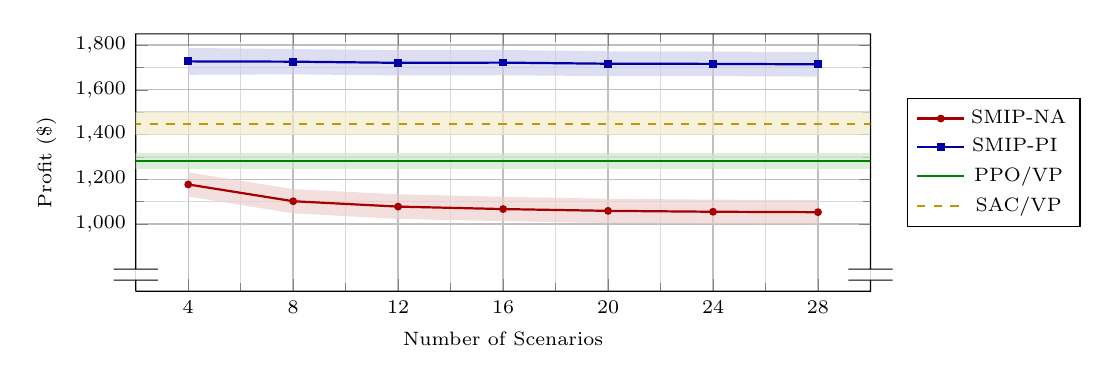
\begin{tikzpicture}
    \begin{axis}[
        width=0.9\textwidth,
        height=0.40\textwidth,
        xlabel={Number of Scenarios},
        ylabel={Profit (\$)},
        legend style={font=\scriptsize,
        at={(1.05,0.5)},  anchor=west,
        legend columns=1,         align=left},
        % under: legend style={font=\scriptsize, at={(0.5,-0.3)}, anchor=north, legend columns=3},
        tick label style={font=\scriptsize},
        label style={font=\scriptsize},
        grid=both,
        minor tick num=1,
        major grid style={line width=.5pt,draw=gray!50},
        minor grid style={line width=.5pt,draw=gray!30},
        ymajorgrids=true,
        yminorgrids=true,
        xtick={0,4,8,...,64},
        xmin=2, xmax=30,
        ymin=700, ymax=1850,
        ytick={1000,1200,..., 1800},
        axis y discontinuity=parallel, % Adds a break in the y-axis
        set layers,
    ]
    SMIP-NA Objective Value
    \addplot[
        color=darkred,
        mark=*,
        mark size=1,
        line width=.8pt
    ] coordinates {
        (4,1177) (8,1102) (12,1078) (16, 1067) (20,1059) (24,1055) (28,1053.02)
    };
    \addlegendentry{SMIP-NA};
        % SMIP-PI Objective Value
    \addplot[
        color=darkblue,
        mark=square*,
        mark size=1,
        line width=.8pt
    ] coordinates {
        (4,1726.94) (8,1725.61) (12,1720.46) (16,1721.39) (20,1716.40) (24,1715.75) (28,1713.73)
    };
    \addlegendentry{SMIP-PI };
    % PPO Objective Value
    \addplot[
        color=darkgreen,
        line width=.8pt
    ] coordinates {
        (0,1283) (40,1283)
    };
    \addlegendentry{PPO/VP};
    % SAC Objective Value
    \addplot[
        dashed,
        color=darkyellow,
        line width=.8pt
    ] coordinates {
        (0,1448) (40,1448)
    };
    \addlegendentry{SAC/VP};
    % Confidence intervals for SMIP-NA
    \addplot[name path=lower_na, draw=none] coordinates {
        (4,1123) (8,1048) (12,1023) (16,1013) (20,1004) (24,1001) (28,999)
    };
    \addplot[name path=upper_na, draw=none] coordinates {
        (4,1231) (8,1156) (12,1133) (16,1122) (20,1113) (24,1109) (28,1107)
    };
    \addplot[darkred!20, opacity=0.65] fill between[of=upper_na and lower_na];
    % Confidence intervals for SMIP-PI
    \addplot[name path=lower_pi, draw=none] coordinates {
        (4,1667) (8,1669) (12,1664) (16,1665) (20,1661) (24,1661) (28,1659)
    };
    \addplot[name path=upper_pi, draw=none,] coordinates {
        (4,1787) (8,1782) (12,1777) (16,1778) (20,1772) (24,1771) (28,1768)
    };
    \addplot[darkblue!20, opacity=0.65] fill between[of=upper_pi and lower_pi];
    % Confidence intervals for PPO
    \addplot[name path=lower_na, draw=none] coordinates {
        (0,1247) (30,1247)
    };
    \addplot[name path=upper_na, draw=none] coordinates {
        (0,1318) (30,1318)
    };
    \addplot[darkgreen!20, opacity=0.70] fill between[of=upper_na and lower_na];
    % Confidence intervals for SAC
    \addplot[name path=lower_na, draw=none] coordinates {
        (0,1397) (30,1397)
    };
    \addplot[name path=upper_na, draw=none] coordinates {
        (0,1499) (30,1499)
    };
    \addplot[darkyellow!20, opacity=0.70] fill between[of=upper_na and lower_na];
    \end{axis}
\end{tikzpicture}
\caption{Profit with 95\% CI across scenario sizes on 30 instances.}

\label{fig:objective_values}
\end{subfigure}

% Subfigure (b): Computational Time Plot
\begin{subfigure}[ht]{0.48\textwidth}
\centering
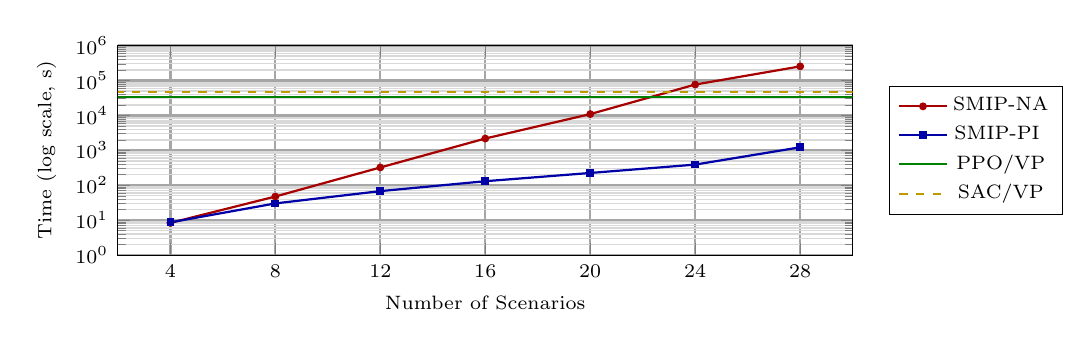
\begin{tikzpicture}
    \begin{axis}[
        width=0.9\textwidth,
        height=0.35\textwidth,
        xlabel={Number of Scenarios},
        ylabel={Time (log scale, s)},
        ymode=log, % Logarithmic scale for y-axis
        legend style=
        {font=\scriptsize,
        at={(1.05,0.5)},  
        anchor=west,
        legend columns=1,
        align=left            
        },
        % under: legend style={font=\scriptsize, at={(0.5,-0.3)}, anchor=north, legend columns=3},
        tick label style={font=\scriptsize},
        label style={font=\scriptsize},
        grid=both, % Show both major and minor grid lines
        major grid style={line width=.8pt, draw=gray!70}, % Thicker and darker for major grid
        minor grid style={line width=.5pt, draw=gray!30}, % Lighter for minor grid
        ymajorgrids=true,
        yminorgrids=true,
        xtick={0,4,...,64},
        xmin=2, xmax=30,
        ymin=1, ymax=1000000,
        ytick={1, 10, 100, 1000, 10000, 100000, 1000000},
        yticklabels={$10^{0}$, $10^{1}$, $10^{2}$, $10^{3}$, $10^{4}$, $10^{5}$, $10^{6}$},
    ]
    % SMIP-NA Computational Time
    \addplot[
        color=darkred,
        mark=*,
        mark size=1,
        line width=.8pt
    ] coordinates {
        (4,8.40) (8,47.70) (12,323.70) (16, 2181.00) (20,10905) (24,76442.7) (28,253037.4)
    };
    \addlegendentry{SMIP-NA};
    % SMIP-PI Computational Time
    \addplot[
        color=darkblue,
        mark=square*,
        mark size=1,
        line width=.8pt
    ] coordinates {
        (4,8.70) (8, 30.30) (12,  68.10) (16,  130.80) (20, 225.30) (24, 391.20) (28, 1222.50)
    };
    \addlegendentry{SMIP-PI };
    % DRL Training Time
    \addplot[
        color=darkgreen,
        line width=.8pt
    ] coordinates {
        (0,33085.9) (40,33085.9)
    };
    \addlegendentry{PPO/VP}
    % DRL Training Time
    \addplot[
        dashed,
        color=darkyellow,
        line width=.8pt
    ] coordinates {
        (0,47988.6) (40,47988.6)
    };
    \addlegendentry{SAC/VP}
    \end{axis}
\end{tikzpicture}
\caption{Total computational time across scenario sizes of 30 instances.}
\label{fig:computational_times}
\end{subfigure}

\begin{subfigure}[ht]{0.48\textwidth}
\centering
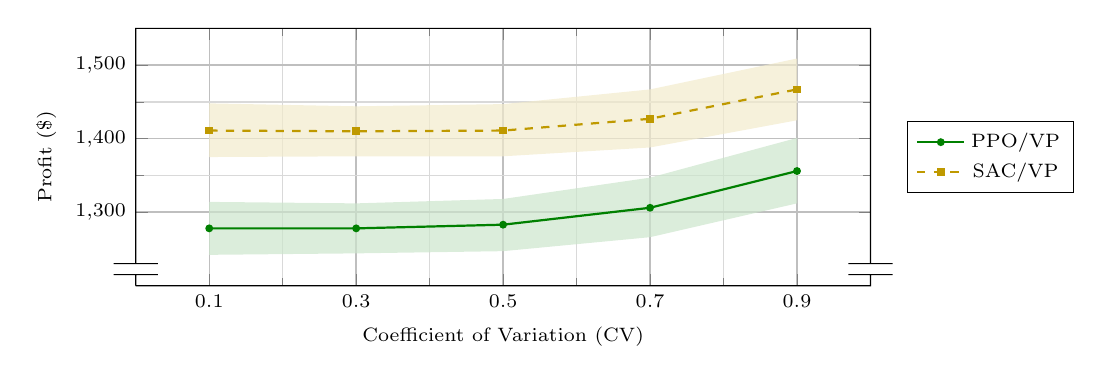
\begin{tikzpicture}
\begin{axis}[
    width=0.9\textwidth,
    height=0.40\textwidth,
    xlabel={Coefficient of Variation (CV)},
    ylabel={Profit (\$)},
    legend style={font=\scriptsize,
    at={(1.05,0.5)},  anchor=west,
    legend columns=1, align=left},
    tick label style={font=\scriptsize},
    label style={font=\scriptsize},
    grid=both,
    minor tick num=1,
    major grid style={line width=.5pt,draw=gray!50},
    minor grid style={line width=.5pt,draw=gray!30},
    ymajorgrids=true,
    yminorgrids=true,
    xtick={0.1,0.3,0.5,0.7,0.9},
    xmin=0, xmax=1,
    ymin=1200, ymax=1550,
    ytick={1300,1400,1500},
    axis y discontinuity=parallel, % Adds a break in the y-axis
]
% PPO/VP
\addplot[
    color=darkgreen,
    mark=*,
    mark size=1,
    mark options={solid},
    line width=.8pt
] coordinates {
    (0.1, 1278) (0.3, 1278) (0.5, 1283) (0.7, 1306) (0.9, 1356)
};

\addlegendentry{PPO/VP};

% SAC/VP
\addplot[
    dashed,
    color=darkyellow,
    mark=square*,
    mark size=1,
    mark options={solid},
    line width=.8pt
] coordinates {
    (0.1, 1411) (0.3, 1410) (0.5, 1411) (0.7,1427) (0.9, 1467)
};
\addlegendentry{SAC/VP};

% PPO-1
\addplot[name path=lower_ci, draw=none] coordinates {
    (0.1, 1242) (0.3, 1244) (0.5,  1247) (0.7, 1266) (0.9, 1312)
};
\addplot[name path=upper_ci, draw=none] coordinates {
    (0.1, 1314) (0.3, 1312) (0.5, 1318) (0.7, 1347) (0.9, 1401)
};
\addplot[darkgreen!20, opacity=0.70] fill between[of=upper_ci and lower_ci];

% SAC-1
\addplot[name path=lower_ci, draw=none] coordinates {
    (0.1, 1375) (0.3, 1376) (0.5, 1376) (0.7, 1388) (0.9, 1425)
};
\addplot[name path=upper_ci, draw=none] coordinates {
    (0.1, 1448) (0.3, 1444) (0.5, 1447) (0.7, 1467) (0.9,1509)
};
\addplot[darkyellow!20, opacity=0.70] fill between[of=upper_ci and lower_ci];

\end{axis}
\end{tikzpicture}
\caption{Profit with 95\% CI across CV levels on 30 unseen instances.}
\label{fig:demand_uncertainty}
\end{subfigure}
\caption{Sensitivity analysis of scenario size and demand spread.}
\label{fig:comparison_subfigures}
\end{figure}

\section{Conclusion and Future Directions}
This work introduces a novel MDP formulation for the MPP under demand uncertainty, incorporating realistic inequality constraints. We train an AM policy using actor-critic DRL methods with differentiable feasibility projections to construct MPP solutions. Experimental results demonstrate that our policy efficiently generates adaptive and feasible solutions, significantly outperforming baseline DRL methods and the SMIP-NA. This approach establishes an AI-driven decision-support policy for planning under uncertainty in a critical part of the global supply chain. Future work will extend the MPP formulation and scale to larger vessels and longer voyages, further enhancing the representativeness.

\clearpage

% \section{Acknowledgements}

\section*{Ethical Statement}
Human oversight is critical in decision-support tools to ensure fairness, accountability, and transparency. While models can enhance decision-making, they must not replace human judgment, particularly in high-stakes applications. We strongly encourage safeguards to mitigate automation bias, ensuring that users can override or challenge outputs, with continuous validation and auditing to uphold trust and fairness.

% \bibliographystyle{plain}
% %%%% ijcai25.tex

\typeout{IJCAI--25 Instructions for Authors}

% These are the instructions for authors for IJCAI-25.

\documentclass{article}
\pdfpagewidth=8.5in
\pdfpageheight=11in

% The file ijcai25.sty is a copy from ijcai22.sty
% The file ijcai22.sty is NOT the same as previous years'
\usepackage{ijcai25}

% Use the postscript times font!
\usepackage{times}
\usepackage{soul}
\usepackage{url}
\usepackage[hidelinks]{hyperref}
\usepackage[utf8]{inputenc}
\usepackage[small]{caption}
\usepackage{graphicx}
\usepackage{amsmath}
\usepackage{amsthm}
\usepackage{booktabs}
\usepackage{algorithm}
\usepackage{algorithmic}
\usepackage[switch]{lineno}

% Comment out this line in the camera-ready submission
% \linenumbers

\urlstyle{same}

% the following package is optional:
%\usepackage{latexsym}

% See https://www.overleaf.com/learn/latex/theorems_and_proofs
% for a nice explanation of how to define new theorems, but keep
% in mind that the amsthm package is already included in this
% template and that you must *not* alter the styling.
\newtheorem{example}{Example}
\newtheorem{theorem}{Theorem}

% Following comment is from ijcai97-submit.tex:
% The preparation of these files was supported by Schlumberger Palo Alto
% Research, AT\&T Bell Laboratories, and Morgan Kaufmann Publishers.
% Shirley Jowell, of Morgan Kaufmann Publishers, and Peter F.
% Patel-Schneider, of AT\&T Bell Laboratories collaborated on their
% preparation.

% These instructions can be modified and used in other conferences as long
% as credit to the authors and supporting agencies is retained, this notice
% is not changed, and further modification or reuse is not restricted.
% Neither Shirley Jowell nor Peter F. Patel-Schneider can be listed as
% contacts for providing assistance without their prior permission.

% To use for other conferences, change references to files and the
% conference appropriate and use other authors, contacts, publishers, and
% organizations.
% Also change the deadline and address for returning papers and the length and
% page charge instructions.
% Put where the files are available in the appropriate places.


% PDF Info Is REQUIRED.

% Please leave this \pdfinfo block untouched both for the submission and
% Camera Ready Copy. Do not include Title and Author information in the pdfinfo section
\pdfinfo{
/TemplateVersion (IJCAI.2025.0)
}

\title{A Survey on Image Quality Assessment:\\ Insights, Analysis, and Future Outlook}


% % Single author syntax
% \author{
%     Author Name
%     \affiliations
%     Affiliation
%     \emails
%     email@example.com
% }

% Multiple author syntax (remove the single-author syntax above and the \iffalse ... \fi here)
% \iffalse
\author{
Chengqian Ma$^1$
\and
Zhengyi Shi$^2$\and
Zhiqiang Lu$^2$\and
Shenghao Xie$^1$\and
Fei Chao$^2$\And
Yao Sui$^1$\\
\affiliations
$^1$National Institute of Health Data Science, Peking University, Beijing, China\\
$^2$School of Informatics, Xiamen University, Xiamen, Fujian, China\\
% \emails
% \{first, second\}@example.com,
% third@other.example.com,
% fourth@example.com
}
% \fi

\begin{document}

\maketitle

\begin{abstract}
Image quality assessment (IQA) represents a pivotal challenge in image-focused technologies, significantly influencing the advancement trajectory of image processing and computer vision. Recently, IQA has witnessed a notable surge in innovative research efforts, driven by the emergence of novel architectural paradigms and sophisticated computational techniques. This survey delivers an extensive analysis of contemporary IQA methodologies, organized according to their application scenarios, serving as a beneficial reference for both beginners and experienced researchers. We analyze the advantages and limitations of current approaches and suggest potential future research pathways. The survey encompasses both general and specific IQA methodologies, including conventional statistical measures, machine learning techniques, and cutting-edge deep learning models such as convolutional neural networks (CNNs) and Transformer models. The analysis within this survey highlights the necessity for distortion-specific IQA methods tailored to various application scenarios, emphasizing the significance of practicality, interpretability, and ease of implementation in future developments.
\end{abstract}

\section{Introduction}
Methods for image quality assessment (IQA) play a critical role in establishing benchmarks to refine algorithms within various domains of computer vision. IQA is crucial to evaluate the efficacy of image processing algorithms, such as dehazing algorithms (DHAs)~\cite{min2019quality}, medical image processing methods~\cite{rosen2018quantitative}, and image deblurring algorithms~\cite{liu2013no}. These algorithms aim to improve image quality, and their success is often demonstrated through the improved quality of the images produced. Previous surveys have organized IQA methods by the availability of a reference image~\cite{5412098}, types of distortions~\cite{Xu2017NoreferenceBlindIQ}, and utilized techniques~\cite{8822415}. However, these surveys fall short in covering the wide range of application scenarios and lag behind the latest innovations. Our study provides an updated review of recent IQA advancements, focusing on different application scenarios to offer a comprehensive overview of the field.

\begin{figure}[t]
    \centering
    \includegraphics[width=0.45\textwidth]{Metric_Struct.pdf}
    \caption{Classification of IQA Methods.}
    \label{fig:metric_struct}
\end{figure}

IQA can be classified into two categories: subjective IQA (SIQA) and objective IQA (OIQA). SIQA relies on human evaluators and is further subdivided by the presence or absence of a reference image. In single stimulus rating~\cite{series2012methodology}, evaluators assign scores based solely on their personal judgment, whereas in double stimulus~\cite{series2012methodology} rating, a reference image is provided for comparison. OIQA is an automated process that excludes human intervention and is typically evaluated using distorted images with corresponding mean opinion scores (MOSs) determined by human evaluation.
Although SIQA is the benchmark due to its high alignment with the human visual system (HVS), it is often deemed impractical for extensive application as it is time-consuming, expensive, and highly subjective. In contrast, OIQA methods are fast and cost-effective. The main challenge lies in developing OIQA techniques to achieve accuracy and reliability comparable to SIQA. OIQA methods are further classified into full-reference (FR), reduced-reference (RR), and no-reference (NR) categories. The NR category, also known as blind image quality assessment (BIQA), has attracted considerable research focus due to the absence of need for reference images in various applications.

Different application scenarios impose distinct requirements on IQA methods. For example, medical imaging prioritizes lesion visibility, while portrait photography emphasizes aesthetics. These varying, and occasionally conflicting, demands call for specialized IQA approaches that are context-specific. This paper initially examines general IQA methods that are applicable in various scenarios before diving into those tailored for particular applications. Table~\ref{tab:abbreviations} lists the specialized terms and their abbreviations used in this paper, while Figure~\ref{fig:metric_struct} depicts the categorization of the IQA methods presented in this survey.% The remainder of this survey is organized as follows. Section 2 presents IQA methods, Section 3 discusses future work, and Section 4 concludes the survey and highlights important future work insights.

% \begin{figure*}[htbp]
%     \centering
%     \includegraphics[width=\textwidth]{Metric Struct.pdf} 
%     \caption{Classification of IQA methods presented in this paper.}
%     \label{fig:metric_struct}
% \end{figure*}

\begin{table}[t]
    \centering
    \begin{tabular}{ll}
        \toprule
        \textbf{Abbreviations} & \textbf{Full Name} \\
        \midrule
        IQA & Image Quality Assessment \\
        SVD & Singular Value Decomposition \\
        % DNT & Divisive Normalization Transform \\
        HVS & Human Visual System \\
        SIQA & Subjective IQA \\
        OIQA & Objective IQA \\
        BIQA & Blind Image Quality Assessment \\
        NAR & Non-Aligned Reference \\
        AR & Aligned Reference \\
        MOS & Mean Opinion Score \\
        CNN & Convolutional Neural Network \\
        GAN & Generative Adversarial Networks \\
        PC & Phase Congruency \\
        GM & Gradient Magnitude \\
        DCT & Discrete Cosine Transform \\
        NSS & Natural Scene Statistics \\
        % TAB & Transposed Attention Block \\
        % SSTB & Scale Swin Transformer Block \\
        HDR & High Dynamic Range \\
        LDR & Low Dynamic Range \\
        TMOs & Tone-Mapped Images Operators \\
        % KNN & K-Nearest-Neighbor \\
        DHA & Dehazing Algorithm \\
        CNR & Contrast-to-Noise Ratio \\
        SNR & Signal-to-Noise Ratio \\
        % LIEAs & Low-Light Image Enhancement \\
        % & Algorithms \\
        ViT & Vision Transformer \\
        \bottomrule
    \end{tabular}
    \caption{Terminology and Abbreviation}
    \label{tab:abbreviations}
\end{table}

\section{Image Quality Assessment Methods}
\subsection{General Scene Methods}
This section outlines the IQA methods applicable to general scenes, divided into two segments: \textit{Statistics Methods} and \textit{Machine Learning-based Methods}.
\subsubsection{Statistics Methods}
Statistics methods predominantly encompass \textit{HVS-based Methods}, \textit{Transform Domain-based Methods}, and \textit{Natural Scene Statistics (NSS)-based Methods}.
\paragraph{HVS-Based Methods}
The fundamental metrics, such as mean squared error (MSE), signal-to-noise ratio (SNR), peak signal-to-noise ratio (PSNR), and universal image quality index (UQI)~\cite{wang2002universal}, evaluate image noise and fidelity based on statistical characteristics and overlook the HVS. This oversight leads to notable discrepancies from human perception. In response, methodologies like Visual SNR (VSNR)~\cite{chandler2007vsnr} and HVS-based PSNR (PSNR-HVS)~\cite{egiazarian2006new} have been developed to incorporate HVS considerations. The Visual Saliency-induced Index (VSI)~\cite{zhang2014vsi} posits that the saliency of each pixel affects its importance, determined by the content of the image. This implies prioritizing the information underlying the image rather than treating every pixel equally. For example, Visual Information Fidelity (VIF)~\cite{sheikh2006image} correlates image quality with the fidelity of image information, using an information-theoretic framework to measure how distortion affects image quality.

In the course of aligning with the HVS, multiple characteristics have been identified and utilized in the design of IQA:

Gradient Magnitude Similarity Deviation (GMSD)~\cite{xue2013gradient} notes that HVS is highly sensitive to edge details, which can be captured by gradient magnitude (GM) for quality assessment. This utilization is also seen in studies such as the perceptual similarity (PSIM)~\cite{gu2017fast}, which measures the similarities of micro- and macro-structures described by GM maps; the gradient similarity (GSIM)~\cite{liu2011image} index, which introduces a measure for gradient similarity; and the feature similarity (FSIM)~\cite{zhang2011fsim} index, which selects phase congruency and gradient deviation (GD) as predictive features of quality.

Structural Similarity (SSIM)~\cite{wang2004image} focuses on the structural information of images, inspired by the HVS's key role in capturing structure within the visual scene~\cite{wang2002image}. To enhance its applicability and efficacy, variants such as multiscale SSIM (MS-SSIM)~\cite{wang2003multiscale} and information content weighted SSIM (IW-SSIM)~\cite{wang2010information} have been proposed.

The HVS employs distinct strategies when processing images of varying qualities. For high-quality images, the HVS focuses more on point-wise variations, rendering metrics like MSE and PSNR appropriate. In the case of lower-quality images, the HVS prioritizes whether the image structure and content remain intact. The Most Apparent Distortion (MAD)~\cite{larson2010most} method addresses this by considering both strategies and weighting their scores according to image quality. Table~\ref{tab:hvs_based} summarizes the HVS-based methods.

\begin{table}
    \centering
    \begin{tabular}{lrr}
        \toprule
        Metric & Citation & Time \\
        \midrule
        SSIM   & 58,352 & 2004.04 \\
        MS-SSIM & 8,043 & 2004.05 \\
        UQI    & 7,419 & 2002.03 \\
        FSIM   & 5,512 & 2011.01 \\
        VIF    & 4,861 & 2006.02 \\
        MAD    & 2,250 & 2010.01 \\
        GMSD   & 1,716 & 2013.12 \\
        VSNR   & 1,578 & 2007.08 \\
        IW-SSIM & 1,533 & 2010.11 \\
        VSI    & 1,082 & 2014.08 \\
        GSIM   & 872  & 2011.11 \\
        % CW-SSIM & 455 & 2005.05 \\
        PSNR-HVS & 433 & 2006.01 \\
        % RR-SSIM & 320 & 2012.08 \\
        PSIM   & 238 & 2017.05 \\
        \bottomrule
    \end{tabular}
    \caption{HVS-based Methods. The citation number is sourced from Google Scholar as of Feb. 1, 2025. The time represents the earliest appearance of the metric.}
    \label{tab:hvs_based}
\end{table}

\paragraph{Transform Domain-Based Methods}
In addition to leveraging features like structural information, edge details, and phase congruency pertinent to the HVS for IQA, images can be transformed into alternative domains where their transformed coefficients serve to characterize the image features.

Singular Value Decomposition (SVD)~\cite{shnayderman2006svd} is used to extract features for IQA at both global and local scales. In addition, methods such as SFF~\cite{chang2013sparse} and QASD~\cite{li2016sparse} employ sparse representation to derive features, while the wavelet transform is utilized in studies such as~\cite{wang2005reduced} to assess images based on changes in wavelet coefficients due to distortion. The Blind Image Integrity Notator using DCT statistics (BLIINDS-II)~\cite{saad2012blind} leverages the statistical properties of coefficients in the discrete cosine transform (DCT) domain, which are affected by distortion, for IQA purposes. Table~\ref{tab:transform_domain} provides an overview of transform domain-based methods.

\begin{table}
    \centering
    \begin{tabular}{lrr}
        \toprule
        Metric & Citation & Time \\
        \midrule
        BLIINDS-II & 1,912 & 2012.03 \\
       ~\cite{wang2005reduced}         & 600  & 2005.03 \\
       ~\cite{shnayderman2006svd}         & 482  & 2006.02 \\
        SFF        & 180  & 2013.06 \\
        QASD       & 50   & 2016.06 \\
        \bottomrule
    \end{tabular}
    \caption{Transform Domain-based Methods. The citation number is sourced from Google Scholar Feb. 1, 2025. The time represents the earliest appearance of the metric.}
    \label{tab:transform_domain}
\end{table}

\begin{table}[b]% [htbp]
    \centering
    \begin{tabular}{lrr}
        \toprule
        Metric & Citation & Time \\
        \midrule
        IFC    & 1,721 & 2005.11 \\
        TMQI   & 720  & 2012.01 \\
       ~\cite{gabarda2007blind}     & 397  & 2007.09 \\
        DRIM   & 371  & 2008.08 \\
        \bottomrule
    \end{tabular}
    \caption{NSS-based Methods. The citation number is sourced from Google Scholar Feb. 1, 2025. The time represents the earliest appearance of the metric.}
    \label{tab:nss_based}
\end{table}

\paragraph{NSS-Based Methods}
Alongside HVS and transform-domain features, intrinsic characteristics of natural images are useful for IQA. Methods such as IFC~\cite{sheikh2005information} analyze the statistical properties of natural images to identify distortions and assess their quality. The anisotropy-based method~\cite{gabarda2007blind} evaluates image quality by examining the variance of the expected entropy in the image, showing high consistency with human visual preferences.

The range of luminance in natural images is another significant area of interest. High dynamic range (HDR) images capture a wide range of luminance levels, but standard displays generally possess a limited dynamic range. To render HDR images on standard devices, Tone-Mapped Image Operators (TMOs) are used to convert HDR images to low dynamic range (LDR) images. Different TMOs produce varying results, and traditional FR-IQA methods are typically limited to image pairs with similar dynamic ranges. The DRIM~\cite{aydin2008dynamic} technique addresses this issue by introducing the High Dynamic Range Visible Differences Predictor (HDR-VDP) model to predict the visibility of contrast differences, effectively handling image pairs with significant dynamic range disparities and broadening the applications of IQA. The Tone-Mapped Image Quality Index (TMQI)~\cite{yeganeh2012objective}, based on SSIM~\cite{wang2004image} and naturalness metrics, achieves a comparable effect. Table~\ref{tab:nss_based} summarizes the NSS-based methods.

\subsubsection{Machine Learning-Based Methods}
This section presents Machine Learning-based Methods, focusing on two perspectives: \textit{Model-based Methods} and \textit{Framework-based Methods}.
\paragraph{Model-based Methods}
We organize Model-based Methods into three categories: \textit{Traditional Machine Learning}, \textit{CNN-based} and \textit{Transformer-based Methods}.
\subparagraph{Traditional Machine Learning Methods}
The advancement of machine learning has led to the implementation of numerous approaches in IQA. For example, methods such as MMF~\cite{liu2012image} and ParaBoost~\cite{liu2015paraboost} integrate multiple quality assessment methods tailored for distinct types of distortion, using SVR to combine scores from multiple quality metrics.

Various machine learning methods employing NSS have been proposed. For example, DIIVINE~\cite{moorthy2011blind} incorporates NSS feature extraction alongside SVM and SVR to identify distortions and evaluate quality.  IL-NIQE~\cite{zhang2015feature} constructs a multivariate Gaussian (MVG) model using NSS features for IQA. BRISQUE~\cite{mittal2012no} achieves multi-scale NSS feature extraction, distortion type analysis, and quality assessment while maintaining minimal computational complexity. Table~\ref{tab:traditional_ml} encapsulates these Traditional Machine Learning Methods.
\begin{table}
    \centering
    \begin{tabular}{lrr}
        \toprule
        Metric & Citation & Time \\
        \midrule
        BRISQUE & 5,733 & 2012.08 \\
        DIIVINE & 2,003 & 2011.01 \\
        IL-NIQE & 1,214 & 2015.04 \\
       % ~\cite{suresh2009no}    & 292  & 2009.03 \\
        MMF    & 216  & 2012.12 \\
       % ~\cite{narwaria2010objective}     & 200  & 2010.01 \\
        SVDR   & 184  & 2011.09 \\
       % ~\cite{wu2015blind}     & 176  & 2015.03 \\
        ParaBoost & 86 & 2015.12 \\
        \bottomrule
    \end{tabular}
    \caption{Traditional Machine Learning Methods. The citation number is sourced from Google Scholar Feb. 1, 2025. The time represents the earliest appearance of the metric.}
    \label{tab:traditional_ml}
\end{table}

\subparagraph{CNN-Based Methods}
Since 2014, when IQA-CNN~\cite{Kang_2014_CVPR} was first introduced, there has been a growing interest in the use of CNNs for IQA. Various CNN techniques have been successfully adapted for IQA, yielding impressive results.~\cite{zhang2018unreasonable} provides experimental evidence showing that deep features outperform alternative metrics. Some notable methods include:

BIECON~\cite{kim2016fully} divides an image into patches and merges their features to compute the quality score, serving as inspiration for subsequent studies.~\cite{bosse2017deep} proposes a completely data-driven method using a Siamese network. MEON~\cite{ma2017end} implements an end-to-end model from image to quality assessment. RankIQA~\cite{liu2017rankiqa} uses a Siamese network to learn the relative ranking of images of different qualities.

In the HVS, the top-down perception model is important for visual tasks, indicating that image content should be understood before IQA. This is because different image contents lead to different evaluation criteria, and the importance of global features can only be determined post image content comprehension. Therefore, a BIQA approach using a Self-Adaptive Hyper Network~\cite{su2020blindly} captures image semantics and constructs a perception rule using a hyper network for IQA.

IQA algorithms must incorporate global and local distortions.~\cite{varga2020multi} leverages the Inception module, which comprises convolutional kernels of various sizes, to interpret visual data at different scales simultaneously. This parallel multi-scale processing is effective since IQA algorithms must address both global structures and local texture details of an image. Since 2020, images generated by Generative Adversarial Networks (GAN) have often exhibited sharper edges and texture-like noises, which are difficult to measure accurately with traditional metrics. Parallel analysis of global and local features can address this issue, with large scales handling global structures and small scales catering to local details. From this perspective, the IQMA Network~\cite{guo2021iqma}, the winner of the NTIRE 21 IQA public leaderboard, proposes a bilateral-branch multi-scale IQA network. The network has two branches that extract multi-scale features from the reference and distorted images, respectively, and features of matching scales from these branches are fed to multiple scale-specific feature fusion modules. Re-IQA~\cite{saha2023re} also tackles this using a dual-encoder Mixture of Experts structure to capture global content alongside local quality of images. In particular, the encoding of global content uses contrastive learning in a creative way.

Most CNN-based FR IQA methods exhibit excessive sensitivity towards texture similarity. DISTS~\cite{ding2020image}is pioneering in its integration of a built-in mechanism for handling texture resampling, effectively combining structural and textural information by leveraging VGG for texture extraction. Table~\ref{tab:cnn_based} summarizes CNN-based methods.
\begin{table}
    \centering
    \begin{tabular}{lrr}
        \toprule
        Metric & Citation & Time \\
        \midrule
        IQA-CNN & 1,406 & 2014.09 \\
       ~\cite{bosse2017deep}     & 1,229 & 2017.10 \\
        DISTS  & 847  & 2020.12 \\
       ~\cite{su2020blindly} & 667 & 2020.06 \\
        MEON   & 593  & 2017.11 \\
        RankIQA & 556  & 2017.07 \\
        BIECON & 487  & 2016.12 \\
       % ~\cite{hou2014blind}    & 433  & 2014.08 \\
        % DeepBIQ & 396  & 2016.02 \\
        % DeepQA & 304  & 2017.10 \\
        % DeepSim & 190  & 2017.09 \\
       % ~\cite{tang2014blind}     & 126  & 2014.09 \\
        Re-IQA & 84   & 2023.04 \\
       ~\cite{varga2020multi} & 44 & 2020.02 \\
        IQMA Network & 27 & 2021.06 \\
        \bottomrule
    \end{tabular}
    \caption{CNN-based Methods. The citation number is sourced from Google Scholar Feb. 1, 2025. The time represents the earliest appearance of the metric.}
    \label{tab:cnn_based}
\end{table}

\begin{table}[ht]
    \centering
    \begin{tabular}{lrr}
        \toprule
        Metric & Citation & Time \\
        \midrule
        MUSIQ & 601 & 2021.08 \\
       ~\cite{golestaneh2022no} & 307 & 2021.08 \\
        Maniqa & 301 & 2022.04 \\
        TRIQ & 230 & 2020.12 \\
        IQT & 167 & 2021.04 \\
        NTIRE 2021 IQA & 114 & 2021.05 \\
        NTIRE 2022 IQA & 113 & 2022.06 \\
        \bottomrule
    \end{tabular}
    \caption{Transformer-based Methods. The citation number is sourced from Google Scholar Feb. 1, 2025. The time represents the earliest appearance of the metric.}
    \label{tab:transformer_based}
\end{table}

\subparagraph{Transformer-Based Methods}
The development of Transformers has heralded a new era in Artificial Intelligence, significantly invigorating IQA. While CNNs necessitate fixed input dimensions for IQA, which requires scaling different-resolution images and leads to data loss, TRIQ~\cite{you2021transformer} uses Transformers to efficiently manage images of different resolutions. The multi-head attention mechanism in the Transformer framework enhances the focus on global features, surpassing the capabilities of CNNs. Building on this, MUSIQ~\cite{ke2021musiq} introduces an innovative method using a hash-based 2D spatial embedding along with a scale embedding. This approach facilitates the processing of images with varying sizes and aspect ratios without necessitating cropping or resizing, which is crucial for IQA applications involving resolution- and aspect-ratio-sensitive images.

Various Vision Transformer (ViT)-based methods have achieved impressive results. For example, the IQT~\cite{cheon2021perceptual} method uses a Siamese architecture to extract features from reference and distorted images, using ViT to evaluate their quality. ViT with relative ranking and self-consistency~\cite{golestaneh2022no} introduces two new losses during the ViT process. The first loss emphasizes the importance of relative image quality scores over absolute scores to better exploit relative ranking information. The second loss addresses the issue of diminished performance in NR-IQA models when images undergo equivariant transformations (e.g., horizontal flipping). Maniqa~\cite{yang2022maniqa} extracts features using ViT and feeds them into the Transposed Attention Block and the Scale Swin Transformer Block, which employ attention mechanisms to analyze features across channels and spatial dimensions.

In the NTIRE 2021 Challenge on Perceptual IQA~\cite{royat2021ntire}, several teams adopted the Transformer framework. The LIPT team pioneered its application to the FR-IQA task. In the following NTIRE 2022 Challenge on Perceptual IQA~\cite{gu2022ntire}, the winners of the FR-IQA and NR-IQA tracks used ViT frameworks, indicating a broad acceptance of ViT-based IQA methods due to their proven effectiveness. Table~\ref{tab:transformer_based} summarizes Transformer-based methods.

\paragraph{Framework-Based Methods}
Besides advancements in model architecture, numerous studies in machine learning focus on developing new training frameworks to address crucial challenges in the IQA field.

Neural networks typically require extensive datasets for effective training, yet numerous specialized IQA tasks face data scarcity. Therefore, CNN-based Medical Ultrasound IQA~\cite{zhang2021cnn} uses transfer learning to leverage the knowledge from existing datasets as a foundation to improve the performance of the Medical Ultrasound IQA model. MetaIQA~\cite{zhu2020metaiqa}, on the other hand, aggregates an extensive dataset featuring various distortion types, mirroring the meta-knowledge that humans use to assess different distortions, which is then applied to evaluate unknown distortion types. UNIQUE~\cite{zhang2021uncertainty}, a BIQA model, demonstrates cross-distortion generalization and proposes a method for simultaneous training on multiple IQA databases. This approach allows the model trained on one distortion type to use knowledge from other distortion types. DeepFL-IQA~\cite{lin2020deepfl} introduces a weakly supervised learning strategy that uses objective IQA metric scores as references during training, with subsequent fine-tuning using subjective quality scores to ensure predictions align with HVS responses, thus mitigating data scarcity issues. CONTRIQUE~\cite{madhusudana2022image} and QAC~\cite{xue2013learning} use self-supervised learning to train on unlabeled images without human scoring. Hallucinated-IQA~\cite{lin2018hallucinated} adopts adversarial learning for NR-IQA. Collectively, these methods effectively tackle the prevalent issue of data scarcity.

A critical issue in NR-IQA research is that CNNs process images pixel-by-pixel without knowing the score for each pixel, in contrast to FR-IQA where each pixel in the reference image is matched with a corresponding pixel for evaluation. Therefore, integrating the knowledge from FR-IQA into NR-IQA is crucial to provide references for each pixel. As a solution,~\cite{kim2018deep} proposes a two-stage training framework. In the initial stage, a CNN predicts an objective error map by comparing reference and distorted images, using the error map as a proxy training target. This approach increases training data and mitigates overfitting. In the second stage, the model is refined to predict human subjective scores. CVRDK-IQA~\cite{yin2022content} accomplishes this using knowledge distillation, which introduces multiple high-quality image priors through non-aligned reference (NAR) images. The disparity in distribution between high- and low-quality images allows the model to better assess image quality. Knowledge distillation transfers this disparity from the FR-teacher to the NAR-student, enabling the student to appreciate the characteristics of high-quality images in the context of IQA. Table~\ref{tab:framework_based} summarizes framework-based methods.
\begin{table}
    \centering
    \begin{tabular}{lrr}
        \toprule
        Metric & Citation & Time \\
        \midrule
        QAC & 470 & 2013.06 \\
        MetaIQA & 405 & 2020.04 \\
       ~\cite{kim2018deep} & 315 & 2018.06 \\
        UNIQUE & 286 & 2021.03 \\
        Hallucinated-IQA & 273 & 2018.04 \\
        CONTRIQUE & 206 & 2022.06 \\
        DeepFL-IQA & 67 & 2020.01 \\
        CVRDK-IQA & 34 & 2022.02 \\
        Medical Ultrasound IQA & 28 & 2021.07 \\
        \bottomrule
    \end{tabular}
    \caption{Framework-based Methods. The citation number is sourced from Google Scholar Feb. 1, 2025. The time represents the earliest appearance of the metric.}
    \label{tab:framework_based}
\end{table}

\begin{table}
    \centering
    \begin{tabular}{lrr}
        \toprule
        Metric & Citation & Time \\
        \midrule
       ~\cite{ferzli2009no} & 1,004 & 2009.04 \\
       ~\cite{rosen2018quantitative} & 360 & 2018.04 \\
        BIBLE & 280 & 2015.01 \\
       ~\cite{min2019quality} & 222 & 2019.02 \\
       ~\cite{liu2013no} & 127 & 2013.11 \\
       ~\cite{gore2015full} & 40 & 2015.02 \\
        % NLIEE & 55 & 2021.06 \\
       ~\cite{chahine2024deep} & 15 & 2024.04 \\
        \bottomrule
    \end{tabular}
    \caption{Specific Scene Metrics. The citation number is sourced from Google Scholar Feb. 1, 2025. The time represents the earliest appearance of the metric.}
    \label{tab:specific_scene}
\end{table}
\subsection{Specific Scene Methods}
Besides the general IQA methods, numerous specialized methods have been developed for specific scenarios. These methods are customized to address the unique demands of their respective applications. Table~\ref{tab:specific_scene} summarizes the Specific Scene Methods.
\subsubsection{Medical IQA}
In brain imaging research, data quality is a significant factor, especially in studies focusing on brain development, where age correlates with data quality.~\cite{rosen2018quantitative} evaluated various quantitative metrics for image quality, including those from the Preprocessed Connectomes Project's Quality Assurance Protocol and the Euler number from FreeSurfer. Among these, the Euler number emerged as the most effective. This result arises because metrics like SNR and Contrast-to-Noise Ratio (CNR) assess global image characteristics, whereas the Euler number examines local topological structures. Local motion artifacts or reconstruction errors may have a minor impact on global metrics but can significantly affect the Euler number. For example, a local motion artifact can create holes or discontinuities in the cortical surface, greatly impacting the Euler number but minimally influencing the SNR or CNR. Consequently, selecting appropriate quality assessment metrics in medical applications should be tailored to specific requirements of the study and the characteristics of the data.
\subsubsection{IQA for Dehazing Algorithms}
DHAs aim to improve image quality in challenging weather conditions like fog by eliminating haze and restoring clarity, contrast, and color, thereby enhancing visual quality and usability. Traditional FR IQA methods fall short in evaluating DHAs effectively because dehazing involves not only image restoration but also contrast enhancement, color adjustment, and structural recovery. These characteristics limit the effectiveness of traditional FR-IQA methods in assessing dehazing outcomes.

~\cite{min2019quality} proposes a method for evaluating dehazing algorithms, emphasizing a holistic approach to image structure restoration, color rendition, and over-enhancement of low-contrast areas comprehensively. This method effectively adapts to the contrast enhancement and color adjustment in dehazing, significantly improving its applicability and accuracy, particularly in the context of aerial images.
\subsubsection{Portrait Quality Assessment}
With the widespread use of smartphones, portrait photography has become ubiquitous, yet assessing the quality of these images remains a challenge. In portraits, the facial region is typically the visual focus, and its quality has a greater impact on overall portrait quality than other areas. Traditional IQA methods usually perform global assessments on the entire image, which fails to adequately emphasize the importance of the facial region. Moreover, portrait quality depends not only on the facial region but also on global factors such as background and composition. Traditional IQA methods often struggle to balance local and global quality assessments simultaneously. Therefore, there is a need for specialized methods to assess portrait quality.

In the NTIRE 2024 Challenge, Deep Portrait Quality Assessment track~\cite{chahine2024deep}, each team introduced unique methods. For example, PQE~\cite{chahine2024deep} proposed a two-branch portrait quality assessment model, focusing separately on the entire image and facial components, thus capturing distinct scene and quality features. SAR~\cite{chahine2024deep} devised a network that integrates scene-adaptive global context and local face-awareness, using a face detector for precise facial localization and employing a ViT to model local facial details and the global image. These methods emphasize separate processing of facial features and the background, providing targeted IQA solutions.
% \subsubsection{IQA for Low Light Enhancement}
% LIEAs aim to improve image quality under low-light conditions by enhancing brightness, contrast, noise reduction, and color modification. Evaluating the effectiveness of these algorithms necessitates a comprehensive assessment method that incorporates various distortion types and complexities. NLIEE~\cite{zhang2021no} stands out as the first NR-IQA metric specifically designed for LIEAs. It evaluates enhanced low-light images by extracting features from four key aspects: lighting enhancement, color contrast, noise measurement, and structural assessment. This specialized approach offers higher accuracy and relevance compared to conventional evaluation methods.
\subsubsection{Specific Distortion}
In computer vision and image processing, image deblurring is a crucial task that aims to recover a sharp image from its blurry counterpart. Blurs can be caused by various factors such as camera shake, object motion, or inaccurate focus. The goal of deblurring algorithms is to eliminate these blurs and restore the original image. However, it is often difficult to perfectly recover the ideal clear image in practice. These algorithms may produce various artifacts that detract from image quality. For example, ringing artifacts (ripple-like structures near edges) are prevalent in deblurring processes and can significantly disrupt human visual perception.

Various deblurring algorithms may produce unique artifact types, each with distinct characteristics. Therefore, a method that can effectively evaluate these artifacts is needed.~\cite{liu2013no} designs a series of features specifically targeting deblurring artifacts, including a new NR method to detect large-scale ringing artifacts; various methods for gauging noise levels in deblurred results; and multiple sharpness metrics for assessing deblurring clarity. These features collectively allow for a thorough assessment of deblurring quality across different artifact types, rather than focusing solely on a single type.

Blurring also causes the attenuation of high-frequency components in images, altering the size of Tchebichef moments. Therefore, BIBLE~\cite{li2015no} calculates gradients to remove low-frequency components, allowing high-frequency components to dominate and more effectively represent blurring. It then uses Tchebichef moments computed from gradient images to assess blur.

Various IQA techniques focus on distinct factors that cause image degradation. For example,~\cite{ferzli2009no} incorporates the perceptual characteristics of HVS directly into a sharpness metric based on Just Noticeable Blur (JNB), achieving alignment of the sharpness measurement with human subjective perception. In JPEG compression, issues like blocking effect and blurring effect require significant attention.~\cite{gore2015full} evaluates the quality of JPEG compressed images, effectively capturing these distortions and outperforming conventional IQA methods.

In summary, a study of the IQA methods in various settings clearly indicates that IQA must meet specific requirements. Therefore, suggesting a universal IQA method that addresses all challenges is impractical. Instead, the focus should shift towards scene-specific IQA, considering the unique demands when designing IQA metrics.

\begin{figure*}[htbp]
    \centering
    \includegraphics[width=\textwidth]{time-early.pdf}
    \caption{Publication Times of HVS-based Methods, Transform Domain-based Methods, NSS-based Methods and Traditional Machine Learning Methods. For methods that span more than one line, we enclose them in [].}
    \label{fig:early}
\end{figure*}

\begin{figure*}[htbp]
    \centering
    \includegraphics[width=\textwidth]{time-later.pdf}
    \caption{Publication Times of CNN-Based Methods, Transformer-Based Methods, Framework-Based Methods, Specific Scene Methods. For methods that span more than one line, we enclose them in [].}
    \label{fig:later}
\end{figure*}

\section{Discussion and Analysis}
Figures~\ref{fig:early} and~\ref{fig:later} provide a chronological overview of the IQA methods discussed in this paper. Over the course of IQA advancement, primary technologies have progressed from basic statistical indices to traditional machine learning methods like SVR-based models, then to deep learning methods such as CNNs, Transformer-based models, and various training frameworks like meta-learning. However, the predominant IQA methods in use continue to be the traditional PSNR and SSIM, primarily due to their straightforward nature  and high interpretability.

In terms of simplicity, using the top-performing ViT-based model for IQA requires researchers to navigate numerous technical challenges in environment setup and model deployment. Regarding interpretability, neural network-based methods function as black boxes, potentially leading to situations where favorable IQA by a ViT-based module in an image generation system might stem from the image aligning with the IQA's scoring preferences rather than the intrinsic quality of the image.

In the development of IQA, it is imperative to recognize that IQA technology must address diverse practical application scenarios and align with user requirements. The evaluation criteria for image quality should be derived from the perspective of image users. For example, assessing the aesthetic value of an image should be approached from an aesthetic point of view, using standards such as composition, lighting, focus control, and color, as suggested by~\cite{luo2008photo}. When evaluating portrait quality, the approach should mirror that of the teams participating in the NTIRE 2024 Portrait Quality Assessment Challenge~\cite{chahine2024deep}, such as PQE, which evaluates the different effects of facial and background components on portrait quality, recommending a two-branch portrait quality assessment model. Similarly, the model from team SECE-SYSU introduces Scene Adaptive Regressors to separately consider different scenes in portrait quality IQA.

Ultimately, proposing a universal IQA method applicable across all scenarios is impractical, as different scenes demand contrasting quality criteria. For example, motion blur might enhance the realism of an image and be desirable in portrait photography, yet it is deemed poor quality in medical diagnostic images. Future development of IQA methods should begin by focusing on the specific application domains, considering the characteristics of images in those fields and the needs of associated algorithms. Simultaneously, it is crucial to ensure that the metrics are user-friendly and highly interpretable to facilitate their application.
\section{Conclusion}
This paper systematically reviews the main research advancements in the field of IQA, covering both general and specific scenarios, and transitioning from traditional methods to advanced deep learning-based techniques. It offers a comprehensive overview of the development of IQA technology. Through the analysis of the strengths and limitations of various methods, it is apparent that despite continuous advancements, the preference still leans towards traditional methods like PSNR and SSIM. This is mainly due to the simplicity and high interpretability of traditional methods. In contrast, although deep learning-based methods excel in performance, they encounter technical barriers and are often less interpretable in practical applications.

Future advances in IQA technology should prioritize specific scenario needs and create specialized IQA methods suited to varied application contexts. In medical imaging, for example, image quality assessment should focus on lesion visibility, whereas in portrait photography, the quality of the facial area significantly influences the overall portrait quality over other regions. Moreover, the application of IQA technology in production practice should align with user requirements, considering the criteria for assessing image quality from the perspective of image users. When assessing image quality, researchers developing dehazing algorithms ought to prioritize factors such as contrast enhancement and color adjustment, whereas those investigating deblurring algorithms need to be particularly attentive to artifacts such as ringing. 

Consequently, advancing IQA technology requires focusing on enhancing performance as well as the practicality, interpretability, and user-friendliness. By aligning the specific requirements of various scenarios with the characteristics of associated algorithms, it is possible to devise more accurate, efficient, and comprehensible IQA methods, thereby facilitating the development and application of IQA technology.
%% The file named.bst is a bibliography style file for BibTeX 0.99c
\bibliographystyle{named}
\bibliography{ijcai25}
\end{document}



\bibliographystyle{named}
\bibliography{references/references.bib} 

\clearpage
\appendix

\section{MDP of Master Planning Problem} \label{app:MDP}

\subsection{Sets and Parameters} \label{app:sets_params}
Provided the sets and parameters in Section \ref{sec:domain}, we introduce additional subsets of the transport set $\textit{TR}$ given port $p \in {P}$:
\begin{itemize}
    \item Onboard transports: $\textit{TR}^{\textit{OB}}_p = \{(i,j)\!\in\!{P}^2\!\mid\! i\leq p, j > p\}$
    \item Arrival transports: $\textit{TR}^{\textit{AC}}_p = \{(i,j)\!\in\!{P}^2\!\mid\! i < p, j > p\}$
    \item Load transports: $\textit{TR}^{{+}}_p = \{(p,j) \!\in\!{P}^2\!\mid\! j > p\}$
    \item Discharge transports: $ \textit{TR}^{{-}}_p = \{(i,p) \!\in\!{P}^2\!\mid\! i < p\}\;$
    \item Transports in crane operations: $\textit{TR}^{M}_p = \textit{TR}^{+}_p \cup \textit{TR}^{-}_p$
\end{itemize}

Considering episode parameters $\zeta$, we define:
\begin{itemize}
    \item Transports: $\textit{tr} = (i,j) \in \textit{TR}$
    \item Cargo types: $k = (\kappa_1, \kappa_2, \kappa_3) \in K$
\end{itemize}

For each combination $(i,j,k)$, we associate the expected demand $\mu^{(i,j,k)}$, standard deviation $\sigma^{(i,j,k)}$, TEU per container $\textit{teu}^{(i,j,k)}$, container weight $w^{(i,j,k)}$, and revenue per container $\textit{rev}^{(i,j,k)}$.

The TEU per container depends on $k$ as:
\[
\textit{teu}(k) =
\begin{cases} 
1, & \text{if } \kappa_1 = \text{20 ft.} \\
2, & \text{if } \kappa_1 = \text{40 ft.}
\end{cases} \; .
\]

Similarly, the container weight is defined by:
\[
\textit{w}(k) =
\begin{cases} 
1, & \text{if } \kappa_2 = \text{Light} \\
2, & \text{if } \kappa_2 = \text{Medium} \\
3, & \text{if } \kappa_2 = \text{Heavy}
\end{cases} \; .
\]

The revenue function is given by:
\[\textit{rev}(i, j, k) =
\begin{cases} 
(j - i)(1 - \textit{LR}) \!+\! 0.1, & \text{if } \kappa_3 = \text{Long} \\
(j - i) \! + \! 0.1, & \text{if } \kappa_3 = \text{Spot}
\end{cases} \; .
\]

The parameters $\mu$ and $\sigma$ are randomly generated, as shown in Appendix \ref{app:gen}. 

\subsection{Formal MDP}
We define the MDP by decomposing the traditional CO problem outlined in \cite{van_twiller_efficient_2024}.

In the traditional MPP, cargo is loaded onto a vessel at each port in a voyage. Let \( u \in \mathbb{R}^{n_u} \) represent the vessel's utilization over the voyage, which is defined by the set of ports \( P = \{1,2,\dots,N_P\} \). Let us also recall the following:
\[
n_u = |B| \times |D| \times |K| \times |\textit{TR}|
\]
\[n_c = |B|\times|D|, \quad n_q = |K|\times |\textit{TR}| \quad n_u = \{n_c \times n_q\}\]

Utilization \( u \) can be decomposed into individual voyage legs, corresponding to the segments between consecutive ports. Specifically, we decompose as:
\[
u = (u_0, u_1, \dots, u_{N_{P-1}})
\]
where each \( u_p \in \mathbb{R}^{n_u} \) represents the vessel's utilization immediately after operations at port \( p \).

\subsubsection{Feasible Region}\label{app:FR_port}
Suppose we have a feasible region for the MPP, where:
\begin{itemize}
    \item \( A' \in \mathbb{R}^{m_u \times n_u} \) is the constraint matrix,
    \item \( b' \in \mathbb{R}^{m_u} \) is the bound vector,
    \item \( u_p \in \mathbb{R}^{n_u}_{\geq 0} \) is the nonnegative vessel utilization.
\end{itemize}
The feasible region, denoted as \( \textit{PH} \), is given by:
\[
\textit{PH}({s}_p) = \{ u_p \in \mathbb{R}^{n_u}_{\geq 0} \mid A' u_p \leq b' \} \;.
\]

At port $p$, utilization can be decomposed into load operations and pre-load utilization:
\[u_p = u'_{p} + u^+_{p} \; ,\]

where:
\begin{itemize}
    \item \( u^+_{p} \in \mathbb{R}^{n_u}_{\geq 0} \) represents load operations,
    \item \( u'_p = u_{p-1} - u^-_{p} \) is the utilization before load operations,
    \item \( u_{p-1} \in \mathbb{R}^{n_u}_{\geq 0} \) is the previous step's utilization,
    \item \( u^-_{p} \in \mathbb{R}^{n_u}_{\geq 0} \) is the discharge operations.
\end{itemize}

Consequently, we can rewrite the feasible region as:
\[
\textit{PH}({s}_p) = \{ u^+_p \in \mathbb{R}^{n_u}_{\geq 0} \mid A' u^+_p \leq b' - A'u'_p \} \;.
\]

\subsection{Decomposed MDP} \label{app:FR_time}
Utilization can be decomposed into sequential steps to refine temporal granularity, thereby obtaining an decomposed MDP formulation. We decompose $u$ as:
\[
u = (u_0, u_1, \dots, u_{T_\textit{seq}})\;,
\]
where \( u_t \in \mathbb{R}^{n_u} \) represents the utilization at time step \( t \), and \( t \in H = \{1,2,\dots,T_\textit{seq}\} \) denotes the episodic horizon \( H \). 

Each step $t$ represents a transport and cargo type, as tuple $(\textit{pol}_t, \textit{pod}_t, k_t)$.  Algorithm \ref{alg:mdp_simulation} illustrates an episode of the decomposed MDP. First, we reset the state \( s_0 \), initialize time \( t \), and an empty trajectory. The episode iterates over load ports (\( \textit{pol}_t \)), discharge ports (\( \textit{pod}_t \)), and cargo classes (\( k_t \)). At each step, we sample action  \( x_t \) from policy \( \pi_{\theta}(x|s_t) \) conditioned on state $s_t$ and episode parameters $\zeta$, and transition to state $s_{t+1}$. Afterwards, we store the results in the trajectory and increment time $t$. This process continues until all combinations of \( \textit{pol}_t \), \( \textit{pod}_t \), and \( k_t \) are explored, accumulating a total of \( T_\textit{seq} \) steps. 

\begin{algorithm}[h]
\caption{Episode of Augmented MDP}
\label{alg:mdp_simulation}
\begin{algorithmic}[1]
\REQUIRE $\mathcal{T}$, $\pi_\theta$, $\zeta$, $\mathcal{Q}$
\STATE $q_{T_\textit{seq}}^{(i,j,k)} \sim \mathcal{Q}(\mu^{(i,j,k)}, \sigma^{(i,j,k)}) \; \forall (i,j) \in \textit{TR}, k \in K$
\STATE $s_0 \gets (\mathbf{0}^{n_u}, q_{T_\textit{seq}} \odot \mathbf{e}^+_0)$, $t \gets 0$, Trajectory $\gets \{\}$
\FOR{$\textit{pol}_t = 1$ to $N_P - 1$}
    \FOR{$\textit{pod}_t = \textit{pol}_t + 1$ to $N_P$}
        \FOR{$k_t \in K$}
            \STATE $x_t \sim \pi_\theta(x | s_t, \zeta)$
            \STATE $s_{t+1} \sim \mathcal{T}(s_t, x_t, \zeta)$
            \STATE Append $(s_t, x_t, r_t, s_{t+1})$ to Trajectory
            \STATE $t \gets t + 1$
        \ENDFOR
    \ENDFOR
\ENDFOR
\RETURN Trajectory
\end{algorithmic}
\end{algorithm}

\subsubsection{Transitions.} 
We use a stochastic transition function \( \mathcal{T}(s_{t+1} | s_t, x_t, \zeta) \in \Delta(S) \). The transition consists of sequential steps:
\begin{enumerate}
     \item If $t \in T_{\text{new port}}$, port demand is revealed. This means we show $q_t^{(i,j,k)} \; \forall (i,j) \in \textit{TR}^+_{\textit{pol}_t}, k\in K$.
    \item If $t \in T_{\text{new port}}$, onboard cargo is discharged \( u_{t+1} = u_t \odot (1 - \mathbf{e}_t^-) \), where \( \mathbf{e}_t^- \in \{0, 1\}^{n_q} \) is a binary mask indicating the cargo type and transport to nullify in \( u_t \).
    \item Each time $t$, cargo is loaded onboard \( u_{t+1} = u_t + x_t \odot \mathbf{e}_t^+ \), where \( \mathbf{e}_t^+ \in \{0, 1\}^{n_q} \) is a binary indicator specifying cargo types and transports to add to \( u_t \).
\end{enumerate}


Additionally, we define the set of time steps before we leave for a new port \( p + 1 \) is defined as follows:
\begin{align*}
T_{\text{leave port}} &= \Big\{ t \in H \ \mid \exists p \in P^{N_P-1}_1 \text{ such that } \\ 
&\qquad\qquad t = |K|\Bigl(p(N_P\!-1\!) - \frac{p(p-1)}{2}\Bigr) - 1 \Big\}.
\end{align*}

Finally, the set of time steps at which we arrive at a new port \( p \) is defined as follows:
\begin{align*}
T_{\text{new port}} &= \Big\{ t \in H \ \mid \exists p \in P^{N_P-1}_1 \text{ such that } \\ 
&\qquad\qquad t = |K|\Bigl((p-1)(N_P\!-1\!) - \frac{p(p-1)}{2}\Bigr) \Big\}.
\end{align*}



\subsubsection{Feasible Region}
The state-dependent feasible region for each time $t$ is formulated as:
\[
\textit{PH}(s_t) = \{ u_t \in \mathbb{R}^{n_u}_{\geq 0} \mid A' u_t \leq b' \}
\]

Similar to the port utilization, utilization can be decomposed into load operations and pre-load utilization:
\[u_t = u'_{t} + u^+_{t}\]
where:
\begin{itemize}
    \item \( u^+_{t} \in \mathbb{R}^{n_u}_{\geq 0} \) represents load operations,
    \item \( u'_t = u_{t-1} - u^-_{t} \) is the utilization before load operations,
    \item \( u_{t-1} \in \mathbb{R}^{n_u}_{\geq 0} \) is the previous step's utilization,
    \item \( u^-_{t} \in \mathbb{R}^{n_u}_{\geq 0} \) is the discharge operations.
\end{itemize}

Using the decomposition, we obtain the feasible region as:
\[
\textit{PH}(s_t) = \{ u_t \in \mathbb{R}^{n_u}_{\geq 0} \mid A' (u^+_t + u'_t) \leq b' \}
\]

\subsubsection{Substituting Load Operations for Actions}
Actions \( x_t \) correspond to transformed load operations \( u^+_t \), given by:
\[
x_t = u^+_{t} M(s_t), \quad M(s_t) \in \{0,1\}^{n_u \times n_c},
\]
where \( M(s_t) \) is a state-dependent sparsity mask that selects relevant elements from \( u^+_t \).

However, load operations are subject to \( m_u \) constraints, whereas actions adhere to \( m_c \) constraints. To bridge this difference, we define the state-dependent constraint matrix:
\[
A(s_t) = T(s_t)^\top A' M(s_t), \quad T(s_t) \in \{0,1\}^{m_u \times m_c},
\]
where:
\begin{itemize}
    \item \( A' \) is the original constraint matrix of shape \( (m_u, n_u) \),
    \item \( T(s_t) \) maps the constraints of \( u_t^+ \) to that of \( x_t \)
    \item \( M(s_t) \) maps the space of \( u_t^+ \) to that of \( x_t \),
\end{itemize}

Similarly, we introduce a state-dependent bound:
\[
b''(s_t) =  T(s_t)^\top b' ,
\]
where:
\begin{itemize}
    \item \( b' \) is the original bound of shape \( (m_u, 1) \),
    \item \( T(s_t) \) maps the constraints of \( u_t^+ \) to that of \( x_t \)
\end{itemize}

\subsubsection{Feasible Region for Actions}
Using the refined notation, we express the state-dependent feasible region in terms of actions:
\[
\textit{PH}(s_t) = \{ x_t \in \mathbb{R}^{n_c}_{\geq 0} \mid A(s_t) x_t \leq b''(s_t) - A'u'_t  \}.
\]

Next, we define the updated bound as:
\[
b(s_t) = b''(s_t) - A' u'_t.
\]

Substituting this into the feasible region, we obtain:
\[
\textit{PH}(s_t) = \{ x_t \in \mathbb{R}^{n_c}_{\geq 0} \mid A(s_t) x_t \leq b(s_t) \}.
\]

\subsection{MPP Constraints}\label{app:mpp_constraints}
Let us specify the MPP constraints of $\textit{PH}({s}_p)$ and $\textit{PH}(s_t)$.

\subsubsection{Demand Constraints} 
Let us consider the demand subset of $\textit{PH}({s}_p)$ as:
\[
\textit{PH}({s}_p)_\text{dem} = \{ {x}_p \in \mathbb{R}^{n_u}_{\geq 0} \mid A'_\text{dem} {x}_p \leq b'_\text{dem} - A'_\text{dem} u'_p \} \;.
\]

We sum over all vessel locations to obtain an aggregated number of containers of shape $n_q$. Note that only current load actions ${x}_p$ are relevant for $q_p$, hence we can omit $ A'_\text{dem} u'_p $ as pre-loading utilization has already satisfied its demand requirements.
\begin{align*}
{x}_p^\top \mathbf{1}_{n_c} & \leq q_p
\end{align*}

Consider the demand subset of $\textit{PH}(s_t)$ as:
\[
\textit{PH}(s_t)_\text{dem} = \{ x_t \in \mathbb{R}^{n_c}_{\geq 0} \mid A(s_t)_\text{dem} x_t \leq b'(s_t)_\text{dem} - A'_\text{dem}u'_t \} \;.
\]

Right now, we can sum the full vector $x_t$ as it needs to sum to scalar $q_t^{(\textit{pol}_t, \textit{pod}_t, k_t)}$. Again, previous steps are irrelevant to demand, hence we can disregard $A'_\text{dem}u'_t$ to obtain:
\begin{align*}
\mathbf{1}^\top x_t & \leq q_t^{(\textit{pol}_t, \textit{pod}_t, k_t)}
\end{align*}

\subsubsection{Capacity Constraints} 
Let us consider the constraint subset of $\textit{PH}({s}_p)$ as:
\[
\textit{PH}({s}_p)_\text{cap} = \{ {x}_p \in \mathbb{R}^{n_u}_{\geq 0} \mid A'_\text{cap} {x}_p \leq b'_\text{cap} - A'_\text{cap} u'_p \} \;.
\]

We sum TEU of all cargo types and transports in ${x}_p$ to obtain TEU use per location with shape $n_c$. The TEU of pre-load utilization is also considered by subtracting it from the vessel capacity, obtaining the following:
\begin{align*}
{x}_p\textit{teu} \leq c - u'_p\textit{teu} \; ,
\end{align*}

Consider the demand subset of $\textit{PH}(s_t)$ as:
\[
\textit{PH}(s_t)_\text{cap} = \{ x_t \in \mathbb{R}^{n_c}_{\geq 0} \mid A(s_t)_\text{cap} x_t \leq b'(s_t)_\text{cap} - A'_\text{cap}u'_t \} \;.
\]

Now, we can do the same trick based on a single scalar $\textit{teu}^{(\textit{pol}_t,\textit{pod}_t, k_t)}$ multiplied with the sum of action $x_t$.
\begin{align*}
\textit{teu}^{(\textit{pol}_t,\textit{pod}_t, k_t)} \mathbf{1}^\top x_t  \leq c - u'_t\textit{teu} \; ,
\end{align*}

\subsubsection{Stability Constraints} 
The stability constraints require some algebra to derive for $\textit{PH}({s}_p)$ and $\textit{PH}(s_t)$.

The lcg constraint in its original form is given by:
\begin{align*}
\frac{\mathbf{1}^\top (\textit{lm} \odot u_p)}{\mathbf{1}^\top(w  \odot u_p)} & \leq \overline{\textit{lcg}} \; .
\end{align*}

Applying the utilization decomposition, we can obtain the formulation for $\textit{PH}({s}_p)$:
\begin{align*}
    \mathbf{1}^\top (\textit{lm} \odot u_p) 
    &\leq \overline{\textit{lcg}} \mathbf{1}^\top (w  \odot u_p) \\
    \mathbf{1}^\top (\textit{lm} \odot u^+_p) 
    + \mathbf{1}^\top (\textit{lm} \odot u'_p) 
    &\leq \overline{\textit{lcg}} \mathbf{1}^\top (w  \odot u^+_p)  \\
    &\quad + \overline{\textit{lcg}} \mathbf{1}^\top (w  \odot u'_p) \\
    \mathbf{1}^\top (\textit{lm}_p \odot {x}_p) 
    - \overline{\textit{lcg}} \mathbf{1}^\top (w \odot {x}_p)  
    &\leq \overline{\textit{lcg}} \mathbf{1}^\top (w  \odot u'_p)  \\
    &\quad - \mathbf{1}^\top (\textit{lm} \odot u'_p) \\
    \;\mathbf{1}^\top \! \big( (\textit{lm}\!-\!\overline{\textit{lcg}} w)\!\odot\!{x}_p \big) & \leq \! \; \mathbf{1}^\top\!\big( (\overline{\textit{lcg}} w\!-\!\textit{lm})\!\odot\!u'_p \big) \;. 
\end{align*}

This approach extends to both the lower and upper bounds for the lcg and vcg, ensuring that vessel stability is properly maintained at every step.

Based on the $\textit{PH}({s}_p)$ constraint, we can substitute load operations for actions, and obtain the formulation for $\textit{PH}(s_t)$:
\begin{align*}
    \;\mathbf{1}^\top \! \big( (\textit{lm}(t) \!-\!\overline{\textit{lcg}} w(t))\!\odot\!x_t \big) & \leq \! \; \mathbf{1}^\top\!\big( (\overline{\textit{lcg}} w\!-\!\textit{lm})\!\odot\!u'_p \big) \;. 
\end{align*}

where $w(t) = w^{(\textit{pol}_t,\textit{pod}_t, k_t)}$ and $\textit{lm}(t) = \textit{lm}^{(\textit{pol}_t,\textit{pod}_t, k_t)}$


\subsection{Auxiliary Variables} \label{app:aux_vars}
The reward function contains two auxiliary variables derived from state $s$,  which incur costs due to inefficient port operations. At port $p$, Equation \eqref{for:hm} creates an indicator of hatch movements $\textit{hm}(s, p) \in \{0,1\}^{|B|}$, whereas Equation \eqref{for:ho} computes the number of on-deck containers during hatch movements, causing hatch overstowage $\textit{ho}(s,p) \in \mathbb{R}^{|B|}_{\geq 0}$.  
\begin{align}
\textit{hm}(s, p) & = \Bigg(\sum_{k \in K} \sum_{\textit{tr} \in \textit{TR}^M_{p}} u_t^{(b,d^\textit{below},k,\textit{tr})} > 0 \Bigg) \label{for:hm} \\ 
\textit{ho}(s, p) & = \textit{hm}(s, p) \Bigg(\sum_{k \in K} \sum_{\textit{tr} \in \textit{TR}^\textit{AC}_{p}} u_t^{(b,d^\textit{above},k,\textit{tr})} \Bigg) \label{for:ho}
\end{align}

Equation \eqref{for:crane_target} computes the target crane moves at port $p$ by equally spreading the total demand per port over pairs of adjacent bays, where $\delta^\textit{cm}$ is the allowed deviation from the equal spread set by ports. Subsequently, Equation \eqref{for:cm} computes the excess crane moves $\textit{cm}(s,p) \in \mathbb{R}^{|B|-1}_{\geq 0}$ 
\begin{align}
\overline{\textit{cm}}(s, p) & = (1 + \delta^\textit{cm}) \frac{2}{|{B}|} \sum_{\textit{tr} \in \textit{TR}^M_{p}} \sum_{k \in {K}} q^{(\textit{tr},k)}_t \label{for:crane_target} \\
{\textit{cm}}(s, p)  & = \max\Bigg(\overline{\textit{cm}}(s, p) - \sum_{d \in D}\sum_{k \in K}\sum_{\textit{tr} \in \textit{TR}^M_{p}} u_t^{(0:|B|-1,d,k,\textit{tr})} \notag \\ &  \qquad \qquad  + u_t^{(1:|B|,d,k,\textit{tr})}, 0\Bigg)\label{for:cm}
\end{align}



\section{Feasibility Mechanisms} \label{app:feas_proj}
Table \ref{tab:feas_implement} provides an overview of implemented feasibility mechanisms.
\begin{table}[h!]
    \centering
    \begin{tabular}{lll}
        \toprule
        \textbf{Type} & \textbf{Implementation} & \textbf{Constraints} \\
        \midrule
        FR  & Composite loss & Constraints $\textit{PH}(s_t)$\\
        VP  & $\textit{VP}(x_t, A(s_t), b(s_t), \alpha_v, \delta_v)$ & Constraints $\textit{PH}(s_t)$\\
        WS  & $\mathcal{W}(x_t, q_t)$ & Demand $q_t$\\
        PC  & $\mathcal{C}(x_t, 0, c- u'_t \textit{teu})$ & TEU capacity $c$\\
        \bottomrule
    \end{tabular}
    \caption{Feasibility mechanisms and relation to constraints}
    \label{tab:feas_implement}
\end{table}

\subsection{Log Probability Adjustments} \label{app:log_prob}
This subsection provides technical details on the adjustments made to the log-probability distribution of the policy as a result of non-linear transformations to distribution samples.

Projecting actions alters the policy's probability density, necessitating consideration of the {change of variables principle} \cite{bishop_pattern_2006}. This principle ensures valid volume scaling by requiring the transformation $f(x)$ to satisfy:
\begin{enumerate}
    \item \textbf{Differentiability}: $f(x)$ must be differentiable to compute the Jacobian $J_f(x)$ and determine local volume scaling.
    \item \textbf{Non-Singularity}: The Jacobian determinant must be non-zero (\( \det(J_f(x)) \neq 0 \)) to prevent dimensional collapse. 
    \item \textbf{Invertibility}: \( f(x) \) must be locally or globally invertible to ensure a one-to-one mapping between points in the original and transformed spaces. 
\end{enumerate}

These properties ensure the transformation is smooth, one-to-one, and well-behaved, enabling the use of the Jacobian adjustment \( \log \pi'(x|s) = \log \pi(x|s) - \log |\det (J_f(x))| \) as a valid probability scaling factor.

\subsubsection{Weighted Scaling Projection Layer.}
Suppose we have variable $x \in \mathbb{R}^n_{>0}$ and scalar $y \in \mathbb{R}_{>0}$ and the following piecewise linear function:
\begin{align*}
\mathcal{P}(x, y) = 
\begin{cases}
x & \text{if } \mathbf{1}^\top{x} \leq y \\
\frac{x}{\mathbf{1}^\top x} \cdot y & \text{if } \mathbf{1}^\top
{x} > y
\end{cases}
\end{align*}

{Case 1: $\mathbf{1}^\top{x} \leq y$}.
\begin{align*}
\mathcal{P}(x, y) & =  x \\
\frac{\partial}{\partial x} \mathcal{P}(x, y) & =  \frac{\partial x}{\partial x} \\
J_\mathcal{P}(x, y) & =  I_n \\
\end{align*}

{Case 2: $\mathbf{1}^\top{x} > y$}, where we apply the product rule and then the quotient rule of differentiation.
\begin{align*}
\mathcal{P}(x, y) & =  \frac{x}{\mathbf{1}^\top x} \cdot y \\
\frac{\partial}{\partial x} \mathcal{P}(x, y) & =  \frac{\partial}{\partial x} \left(\frac{x}{\mathbf{1}^\top x} \cdot y\right) \\
\frac{\partial}{\partial x} \mathcal{P}(x, y) & =  \frac{\partial}{\partial x} \left(\frac{x}{\mathbf{1}^\top x} \right) \cdot y \\
J_\mathcal{P}(x, y) & =  y \cdot\frac{1}{(\mathbf{1}^\top x)^2} \left(I_n \mathbf{1}^\top x - x \cdot \mathbf{1}^\top  \right)  \\
J_\mathcal{P}(x, y) & =  \frac{y \cdot I_n}{(\mathbf{1}^\top x)} - \frac{y \cdot x^\top }{(\mathbf{1}^\top x)^2}
\end{align*}

We obtain the following Jacobian of function $\mathcal{P}(x, y)$: 
\begin{align*}
J_\mathcal{P}(x, y) = 
\begin{cases}
I_n & \text{if } \mathbf{1}^\top{x} \leq y \\
\frac{y}{(\mathbf{1}^\top x)^2} \left(I_n\mathbf{1}^\top x - x 1^\top \right)
& \text{if } \mathbf{1}^\top{x} > y
\end{cases}
\end{align*}

Finally, we verify that Jacobian adjustment is allowed for the weighted scaling projection by: \\
\begin{enumerate}
    \item \( \mathcal{P}(x, y)\) has been shown to be differentiable.
    \item Provided that $x,y > 0$, either case is positive definite as the diagonal elements are strictly positive. We obtain $\det(J_\mathcal{P}(x, y)) > 0$, thus the Jacobian in non-singular.   
    \item \( \mathcal{P}(x, y) \) is locally invertible as \( \det(J_\mathcal{P}(x, y)) \neq 0 \).
\end{enumerate} 

\subsubsection{Violation Projection Layer.} 
Suppose we have function $\mathcal{P}(x, A, b) = x - \eta_v A^\top(Ax - b)_{>0}$ with $x \in \mathbb{R}^n_{>0}$, $\eta_v \in \mathbb{R}_{>0}$, $A \in \mathbb{R}_{\geq 0}^{m\times n}$, $b \in \mathbb{R}^m_{\geq 0}$, and $m > n$. \\

Case 1: $\eta_v A^\top(Ax - b) = 0$.
\begin{align*}
\mathcal{P}(x, A, b) & = x \\ 
\frac{\partial}{\partial x}\mathcal{P}(x, A, b) & = \frac{\partial x}{\partial x} \\ 
J_\mathcal{P}(x, A, b) & = I_n
\end{align*}

Case 2: $\eta_v A^\top(Ax - b) > 0$, where we apply the chain rule on the second term.
\begin{align*}
\mathcal{P}(x, A, b) & = x - \eta_v A^\top(Ax - b) \\ 
\frac{\partial}{\partial x}\mathcal{P}(x, A, b) & = \frac{\partial}{\partial x}\left(x - \eta_v A^\top(Ax - b) \right) \\ 
J_\mathcal{P}(x, A, b) & = I_n -  \eta_v A^\top A
\end{align*}

Both cases are combined in the following matrix formulation with diagonal matrix $\text{Diag} = \text{diag}((Ax - b) > 0)$:
\begin{align*}
J_\mathcal{P}(x, A, b) & = I_n -  \eta_v A^\top \text{Diag} A
\end{align*}

Finally, we can confirm that Jacobian adjustment is allowed for the violation projection layer by:
\begin{enumerate}
    \item $\mathcal{P}(x, A, b)$ is differentiable as shown above. 
    \item Due to the full rank nature of the identity $I_n$ and $A^\top \text{Diag} A$ when $\text{Diag} = I_m$, we get $\det(J_\mathcal{P}(x, A, b)) \neq 0$, and hence the Jacobian is non-singular.
    \item $\mathcal{P}(x, A, b)$ is locally invertible as $\det(J_\mathcal{P}(x,A,b)) \neq 0$. It is not globally invertible, due to the piece-wise nature of $(Ax - b)_{>0}$. 
\end{enumerate}

\subsubsection{Policy Clipping}
We can implement a clipped Gaussian distribution that enforces element-wise bounds on a standard Gaussian \cite{fujita_clipped_2018}. Let $ \mu_\theta $ and $ \sigma^2_\theta $ denote the policy’s mean and variance, with bounds $ \textit{lb}_\textit{pc} $ and $ \textit{ub}_\textit{pc} $, and $ \Phi(\cdot) $ being the cumulative distribution function of the standard Gaussian. Actions are sampled from $ \mathcal{N}(\mu_\theta, \sigma^2_\theta) $ and clipping the result to $[\textit{lb}_\textit{pc}, \textit{ub}_\textit{pc}]$. Provided this transformation, we compute the log probabilities $ \log \pi(x|s) $ for action $ x $ by:
\begin{align*}
\log \pi(x|s) =
\begin{cases}
\log \Phi\left(\frac{\textit{lb}_\textit{pc} - \mu_\theta}{\sigma_\theta}\right) & \text{if } x \leq \textit{lb}_\textit{pc}, \\
-\frac{(x - \mu_\theta)^2}{2\sigma^2_\theta} - \log(\sqrt{2 \pi \sigma^2_\theta}) & \text{if } \textit{lb}_\textit{pc} < x < \textit{ub}_\textit{pc}, \\
\log \left(1 - \Phi\left(\frac{\textit{ub}_\textit{pc} - \mu_\theta}{\sigma_\theta}\right) \right) & \text{if } x \geq \textit{ub}_\textit{pc}
\end{cases}
\end{align*}

\subsection{Violation Projection Layer}
We define a feasible region of action \( x \) as the polyhedron:
\[
\textit{PH} = \{x \in \mathbb{R}^n : Ax \leq b, x \geq 0\},
\]
where $A \in \mathbb{R}^{m\times n}$ and $b \in \mathbb{R}^{m}$.

Constraints in \( \textit{PH} \) may be violated during optimization. To quantify these violations, we introduce the violation function:
\[
\mathcal{V}(x) = (Ax - b)_{>0},
\]
where \( \mathcal{V}(x)_{m_i} > 0 \) indicates that constraint \( {m_i} \) is violated, and \( \mathcal{V}(x)_{m_i} = 0 \) means the constraint is satisfied.

\textbf{Violation Gradient Descent.} To minimize constraint violations, we update \( x \) for a fixed number of iterations using gradient descent on the violation term \( \|\mathcal{V}(x)\|_2^2 \), which represents the squared distance to feasibility. Differentiating with respect to \( x \), we derive the update rule:
\begin{align*}
    x' &= x - \eta_v \nabla_x \|\mathcal{V}(x)\|_2^2  \\
       &= x - \eta_v 2 A^\top \mathcal{V}(x).
\end{align*}
Since the step size \( \eta_v \in (0,1) \) is a tunable parameter, we simplify the update function to:
\[
x' = x - \eta_v A^\top \mathcal{V}(x).
\]

\begin{theorem}[Convergence of Violation Gradient Descent]
Let \( x_0 \in \mathbb{R}^n \) be an initial point, and consider update:
\[
x_{k+1} = x_k - \eta_v A^\top \mathcal{V}(x_k),
\]

where:
\begin{itemize}
    \item \( \mathcal{V}(x) = \max(0, Ax - b) \) is the element-wise function onto nonnegative constraint values.
    \item \( \eta_v \in (0,1) \) is a step size parameter.
    \item \( A \in \mathbb{R}^{m \times n} \) has full row rank.
    \item The feasible region \( \textit{PH} = \{x \in \mathbb{R}^n : Ax \leq b, x \geq 0\} \) is nonempty.
\end{itemize}

Then, the sequence \( \{x_k\} \) satisfies:
\begin{enumerate}
    \item The function \( g(x) = \|\mathcal{V}(x)\|_2^2 \) is non-increasing.
    \item \( x_k \) converges to a feasible point \( x^* \) or a local minimum violation point.
\end{enumerate}
\end{theorem}

\begin{proof}
Define the violation function:
\[
g(x) = \|\mathcal{V}(x)\|_2^2.
\]

Since \( \mathcal{V}(x) \) is an elementwise projection onto nonnegative values, and some function $h(y) = \max(0,y)$ is convex and non-decreasing, then the function \( g(x) = \|\mathcal{V}(x)\|_2^2 \) is convex when \( Ax - b \) is affine.

We apply gradient descent on \( g(x) \) using the update rule:
\[
x_{k+1} = x_k - \eta_v \nabla_x g(x_k).
\]

By the standard descent lemma \cite{boyd_convex_2004}, for a sufficiently small step size \( \eta_v \), we have:
\[
g(x_{k+1}) \leq g(x_k) - \eta_v \|\nabla_x g(x_k)\|_2^2.
\]

Since \( \eta_v > 0 \) and \( \|\nabla_x g(x_k)\|_2^2 \geq 0 \), it follows that:
\[
g(x_{k+1}) \leq g(x_k).
\]

Thus, \( g(x_k) \) is non-increasing. \\

Since \( g(x_k) \) is also lower-bounded by \( 0 \), it must converge to some limit \( g^* \geq 0 \). This implies:
\[
\lim_{k \to \infty} \|\mathcal{V}(x_k)\|_2 = \Tilde{c}, \quad \text{for some } \Tilde{c} \geq 0.
\]


If \( \Tilde{c} = 0 \), then \( x_k \) converges to a feasible point, meaning \( \mathcal{V}(x_k) = 0 \). If \( \Tilde{c} > 0 \), then \( x_k \) converges to a local minimum of \( g(x) \), where no further descent is possible, satisfying \(\nabla_x g(x_k) = 0, \) which implies \(A^\top \mathcal{V}(x_k) = 0.\)
\end{proof}

\section{Instance Generator} \label{app:gen}
During training, we simulate problem instances based on a Gaussian distribution with element $i$:
\[
q^{(i,j,k)} \sim \mathcal{N}\big(\mu^{(i,j,k)}, \sigma^{(i,j,k)}\big) \; \forall (i,j) \in \textit{TR}, k \in K.
\]
Here, \(\mu\) is the expected value of cargo demand, initialized by a uniform generator \(\mathcal{U}(\textit{lb}, \textit{ub})\), while the standard deviation of demand is defined as \(\sigma^{(i,j,k)} = \textit{CV} \cdot \mu^{(i,j,k)}\), where the coefficient of variation (CV) controls the spread of each element based on \(\mu^{(i,j,k)}\). Note that CV is normally defined as
\(\textit{CV}^{(i,j,k)} = \frac{\sigma^{(i,j,k)}}{\mu^{(i,j,k)}}\), so we use \(\sigma^{(i,j,k)} = \textit{CV} \cdot \mu^{(i,j,k)}\) to control the spread of the distribution.

We initialize $\mu^{(i,j,k)} \sim \mathcal{U}(0,\overline{\mu^{(i,j,k)}}) $, where the upper bound on the expected value is found as follows:
\[
\overline{\mu} = \frac{2 \textit{UR} \cdot \mathbf{1}^\top c}{\textit{NC}} \qquad,
\]
where $\textit{UR}$ is the rate of total utilization present in the demand (e.g., 1.2 means total demand is 120\% of total capacity), and $\textit{NC} \in \mathbb{R}^{|TR|}_{>0}$ is a matrix to spread the demand over different elements proportional to the number of transports remaining to be loaded.  

During generalization testing, we simulate problem instances based on a continuous uniform generator:
\[q^{(i,j,k)} \sim \mathcal{U}(\textit{lb}^{(i,j,k)}, \textit{ub}^{(i,j,k)}).\]

To ensure similar mean and variance of the instances, we derive parameters $a$ and $b$ from the definition of the continuous uniform distribution, as follows:
\begin{align*}
\mu^{(i,j,k)} = (\textit{lb}^{(i,j,k)} + \textit{ub}^{(i,j,k)}) / 2 \\
(\sigma^{(i,j,k)})^2 = (\textit{ub}^{(i,j,k)} - \textit{lb}^{(i,j,k)})^2 / 12
\end{align*}

We rewrite to:
\begin{align*}
\textit{lb}^{(i,j,k)} = \mu^{(i,j,k)} - \sqrt{(12 (\sigma^{(i,j,k)})^2)/2}\\
\textit{ub}^{(i,j,k)} = \mu^{(i,j,k)} + \sqrt{(12 (\sigma^{(i,j,k)})^2)/2}
\end{align*}


\section{Multi-stage Stochastic MIP} \label{app:smip}
\subsection{Multi-stage Scenario Tree}
A scenario tree is a directed tree represented as \(T_\textit{ST} = (V_\textit{ST}, E_\textit{ST})\), where \( V_\textit{ST} \) is the set of nodes, each corresponding to a decision or uncertainty realization at a given stage. \( E_\textit{ST} \subseteq V_\textit{ST} \times V_\textit{ST} \) is the set of directed edges representing transitions between nodes over time. 

The tree consists of:  
\begin{enumerate}
    \item A root node \( v_1 \in V_\textit{ST} \), representing the initial state at the first port. 
    \item Stages \( p = 1, 2, \dots, N_{P}-1 \), where each node \( v \) belongs to a stage \( p(v) \). We denote stages by $p$, as stages are equivalent to ports in a voyage.   
    \item Branching structure, where each node has child nodes that correspond to possible future realizations.
    \item A probability measure \( P: V_\textit{ST} \to [0,1] \) assigning probabilities to nodes, ensuring:     \[
   \sum_{v' \in \text{child}(v)} \mathbb{P}(v') =  \mathbb{P}(v), \quad \forall v \in V_\textit{ST}.
   \]  
   \item Scenario paths $\phi \in \mathcal{Z}$, which are root-to-leaf paths representing possible realizations of uncertainty over time.  
\end{enumerate}

\subsection{MIP Formulation}
We define the MPP under demand uncertainty as a multi-stage stochastic MIP. 

\textbf{Decision Variables.} The following variables are included:
\begin{itemize}
    \item Vessel utilization: $\Tilde{u}^{b,d,\phi}_{\textit{tr},k} \in \mathbb{Z}_{\geq0}$
    \item Hatch overstowage: $\Tilde{\textit{ho}}^{\phi}_{p,b} \in \mathbb{Z}_{\geq0}$
    \item Makespan of cranes: $\Tilde{\textit{cm}}^{\phi}_{p} \in \mathbb{Z}_{\geq0}$
    \item Hatch movement: $\Tilde{\textit{hm}}^{\phi}_{p,b} \in \{0,1\}$
\end{itemize}

In addition, we introduce the big $M$ as a sufficiently large constant used to enforce logical constraints. 

\textbf{Objective.} The objective function \eqref{for:MIP_obj} maximizes the revenue and minimizes hatch-overstowage and crane moves costs over scenario paths $\phi \in \mathcal{Z}$ each with probability $\mathbb{P}_\phi$. We assume each scenario path has equal probability.

\textbf{Constraints.} Constraint \eqref{for:MIP_demand} enforces that the onboard utilization cannot exceed the cargo demand $q$, whereas Constraint \eqref{for:MIP_capacity} limits each vessel location to the TEU capacity $c$ for each bay $b \in B$ and deck $d \in D$. In Constraint \eqref{for:hatch}, we indicate that hatches need to be opened if below deck cargo needs to be loaded or discharged. Based on these movements, Constraint \eqref{for:hatch_restow} models the amount of hatch overstowage in containers. Subsequently, we compute the target of crane moves $\overline{z}$ in Constraint \eqref{for:z_upper}, after which Constraint \eqref{for:long_crane} computes the excess number of crane moves $\Tilde{\textit{cm}}$.

Additionally, we model the longitudinal and vertical stability in Constraints \eqref{for:lm} until \eqref{for:VS1}. First, we compute the longitudinal moment, vertical moment and total weight in Constraints \eqref{for:lm}, \eqref{for:vm} and \eqref{for:TW}, respectively. Second, Constraint \eqref{for:LS1} bounds \textit{lcg} between $\underline{\textit{lcg}}$ and $\overline{\textit{lcg}}$. Third,  Constraint \eqref{for:VS1} bounds \textit{vcg} between $\underline{\textit{vcg}}$ and $\overline{\textit{vcg}}$. Both \textit{lcg} and \textit{vcg} are linearized equivalents of the original Constraints \eqref{for:lcg} and \eqref{for:vcg}, respectively. Furthermore, we include non-anticipation in Constraint \eqref{for:nonanti} to prevent leveraging future demand realizations.
\begin{align}
\text{max } & 
\sum_{\phi \in \mathcal{Z}} \mathbb{P}_\phi \sum_{p\in {P}} \sum_{b \in{B}}\sum_{d\in {D}} \sum_{k\in {K}}\sum_{\textit{tr} \in \textit{TR}^\textit{+}(p)} f_1 \Tilde{u}^{b,d,\phi}_{\textit{tr},k} \nonumber \\ 
& \qquad\qquad\qquad\qquad\qquad - f_2 \Tilde{\textit{ho}}^{\phi}_{p,b} - f_3 \Tilde{\textit{cm}}^{\phi}_{p}  \label{for:MIP_obj}
\end{align}
\begin{align}
    \text{s.t. } & 
    \sum_{b \in {B}} \sum_{d \in {D}} \Tilde{u}^{b,d,\phi}_{\textit{tr},k} \leq q^{\phi}_{\textit{tr},k} \nonumber\\
    & \qquad\qquad\qquad \forall p \in {P},\; \textit{tr} \in \textit{TR}^\textit{OB}(p),\; k \in {K},\; \phi \in \mathcal{Z} \label{for:MIP_demand} \\
    & \sum_{k \in {K}} \sum_{\textit{tr} \in \textit{TR}^\textit{OB}(p)} \textit{teu}_{\textit{tr},k} \Tilde{u}^{b,d,\phi}_{\textit{tr},k} \leq c_{b,d} \nonumber\\
    & \qquad\qquad\qquad \forall p \in {P},\; b \in{B},\; d \in {D},\; \phi \in \mathcal{Z} \label{for:MIP_capacity} \\
    & \sum_{k \in {K}} \sum_{\textit{tr} \in \textit{TR}^{M}(p)} \Tilde{u}^{b,d_h,\phi}_{\textit{tr},k} \leq M \Tilde{\textit{hm}}^{\phi}_{p,b} \nonumber\\
    & \qquad\qquad\qquad \forall p \in {P},\; b \in{B},\; \phi \in \mathcal{Z} \label{for:hatch} \\
    & \sum_{k \in {K}} \sum_{\textit{tr} \in \textit{TR}^\textit{AC}(p)} \Tilde{u}^{b,d_o,\phi}_{\textit{tr},k} - M(1 - \Tilde{\textit{hm}}^{\phi}_{p,b}) \leq \Tilde{\textit{ho}}^{\phi}_{p,b} \nonumber\\
    & \qquad\qquad\qquad \forall p \in {P},\; b \in{B},\; \phi \in \mathcal{Z} \label{for:hatch_restow} \\
    & {\overline{z}}^{\phi}_{p} = (1 + \delta^\textit{cm}) \frac{2}{|{B}|} \sum_{\textit{tr} \in \textit{TR}^M(p)} \sum_{k \in {K}} q^{\phi}_{\textit{tr},k} \nonumber\\
    & \qquad\qquad\qquad \forall p \in {P},\; \phi \in \mathcal{Z} \label{for:z_upper} \\
    & {\overline{z}}^{\phi}_{p} - \sum_{b \in{b'}} \sum_{d \in {D}} \sum_{k \in {K}} \sum_{\textit{tr} \in \textit{TR}^{M}(p)} \Tilde{u}^{b,d,\phi}_{\textit{tr},k} \leq \Tilde{\textit{cm}}^{\phi}_{p} \nonumber\\
    & \qquad\qquad\qquad \forall p \in {P},\; {b'} \in {B}',\; \phi \in \mathcal{Z} \label{for:long_crane} \\
    & \textit{tw}^{\phi}_{p} = \sum_{k \in {K}} w_k \sum_{\textit{tr} \in \textit{TR}^\textit{OB}(p)} \sum_{d \in {D}} \sum_{b \in{B}} \Tilde{u}^{b,d,\phi}_{\textit{tr},k} \nonumber\\
    & \qquad\qquad\qquad \forall p \in {P},\; \phi \in \mathcal{Z} \label{for:TW} \\
    & \textit{lm}^{\phi}_{p} = \sum_{b \in{B}} \textit{ld}_b \sum_{k \in {K}} w_k \sum_{\textit{tr} \in \textit{TR}^\textit{OB}(p)} \sum_{d \in {D}} \Tilde{u}^{b,d,\phi}_{\textit{tr},k} \nonumber\\
    & \qquad\qquad\qquad \forall p \in {P},\; \phi \in \mathcal{Z} \label{for:lm} \\
    & \textit{vm}^{\phi}_{p} = \sum_{d \in {D}} \textit{vd}_d \sum_{k \in {K}} w_k \sum_{\textit{tr} \in \textit{TR}^\textit{OB}(p)} \sum_{b \in{B}} \Tilde{u}^{b,d,\phi}_{\textit{tr},k} \nonumber\\
    & \qquad\qquad\qquad \forall p \in {P},\; \phi \in \mathcal{Z} \label{for:vm} \\
    & \underline{\textit{lcg}} \textit{tw}^{\phi}_{p} \leq \textit{lm}^{\phi}_{p} \leq \overline{\textit{lcg}} \textit{tw}^{\phi}_{p} \nonumber\\
    & \qquad\qquad\qquad \forall p \in {P},\; \phi \in \mathcal{Z} \label{for:LS1} \\
    & \underline{\textit{vcg}} \textit{tw}^{\phi}_{p} \leq \textit{vm}^{\phi}_{p} \leq \overline{\textit{vcg}} \textit{tw}^{\phi}_{p} \nonumber\\
    & \qquad\qquad\qquad \forall p \in {P},\; \phi \in \mathcal{Z} \label{for:VS1} \\
    & \Tilde{u}^{b,d,\phi'}_{\textit{tr},k} = \Tilde{u}^{b,d,\phi}_{\textit{tr},k} \nonumber\\
    & \qquad\qquad\qquad \forall p \in {P}, \textit{tr} \in \textit{TR}^{+}(p), k \in {K},\nonumber\\
    & \qquad\qquad\qquad b \in{B}, d \in {D}, \phi, \phi' \in \mathcal{Z} \mid q^{\phi}_{[p-1]} = q^{\phi'}_{[p-1]} \label{for:nonanti}
\end{align}



\section{Deep RL Implementation Details} \label{app:DRL}
To prevent confusion, we 

\subsection{PPO Algorithm} 
PPO is an on-policy reinforcement learning algorithm that seeks to maximize expected cumulative reward while enforcing stable policy updates via clipped importance sampling \cite{schulman_proximal_2017}, as outlined in Algorithm \ref{alg:ppo}. The agent collects trajectories, computing \(n_\text{ppo}\)-step return to evaluate performance with \( V_{\theta}(s) \) as estimated state value:
\begin{equation}
G_t^{(n_\text{ppo})} = \sum_{k_\text{ppo}=0}^{n_\text{ppo}-1} \gamma^k r_{t+k_\text{ppo}} + \gamma^{n_\text{ppo}} V_{\theta}(s_{t+n_\text{ppo}}),  
\label{for:n_return}
\end{equation}

To reduce variance, we adopt Generalized Advantage Estimation (GAE) \cite{schulman_high-dimensional_2016}:
\begin{align}
\hat{A}_t^{\text{GAE}} &= \sum_{l_\text{ppo}=0}^{\infty} (\gamma \lambda)^{l_\text{ppo}} \delta_{t+l_\text{ppo}}, \label{for:gae1} \\ 
\delta_t &= r_t + \gamma V_{\theta}(s_{t+1}) - V_{\theta}(s_t). \label{for:gae2}
\end{align}
Here, \( \delta_t \) is the temporal difference (TD) residual, which quantifies the advantage of taking action \( x_t \) at state \( s_t \).

The actor is updated using the PPO clipped surrogate loss:
\begin{align}
\mathcal{L}_{\text{actor}}(\theta) &= \mathbb{E}_t \Big[ \min \big( \text{ratio}_t(\theta) \hat{A}_t^{\text{GAE}}, \notag \\ 
& \quad \text{clip}(\text{ratio}_t(\theta), 1 - \epsilon, 1 + \epsilon) \hat{A}_t^\text{GAE} \big) \Big], \label{for:ppo_actor}
\end{align}
where the probability ratio is defined as:
\begin{equation}
\text{ratio}_t(\theta) = \frac{\pi_{\theta}(x_t | s_t)}{\pi_{\theta_{\text{old}}}(x_t | s_t)}.
\end{equation}

The critic aims to minimize the squared TD error:
\begin{equation}
\mathcal{L}_{\text{critic}}(\theta) = \mathbb{E}_t \Big[ \big( V_{\theta}(s_t) - G_t^{(n_\text{ppo})} \big)^2 \Big]. 
\label{for:ppo_critic}
\end{equation}

Finally, the total PPO objective, including feasibility regularization from Equation \eqref{for:feas_loss}, is given by:
\begin{align}
\mathcal{L}(\theta) &= \mathcal{L}_{\text{actor}}(\theta) + \lambda_c \mathcal{L}_{\text{critic}}(\theta)  + \lambda_f \mathcal{L}_\text{feas}(\theta) \notag \\ & \qquad - \lambda_e \mathbb{E}_t\big[ \text{entropy}(\pi_{\theta}) \big], 
\label{for:ppo_total_loss}
\end{align}
where \( \lambda_c \), \( \lambda_f \), and \( \lambda_e \) are weighting coefficients for the critic loss, feasibility regularization, and entropy regularization respectively.

\begin{algorithm}
\caption{Proximal Policy Optimization (PPO)}
\label{alg:ppo}
\begin{algorithmic}[1]
\REQUIRE Model parameters $\theta$, steps $n$, learning rate $\eta$
\FOR{each gradient update}
    \FOR{each step $t$}
        \STATE Collect $n$-step trajectories $\{(s_t, x_t, r_t, s_{t+1})\}$
        \STATE Compute $n$-step returns $G_t^{(n_\text{ppo})}$
        \STATE Compute advantage estimates $\hat{A}_t^{\text{GAE}}$
    \ENDFOR
    \STATE Update parameters: $\theta \gets \theta + \eta \nabla_{\theta} \mathcal{L}(\theta)$
\ENDFOR
\RETURN Policy $\pi_\theta$
\end{algorithmic}
\end{algorithm}

\subsection{SAC Algorithm}  
Soft Actor-Critic (SAC) is an off-policy reinforcement learning algorithm that optimizes both reward maximization and entropy to encourage efficient exploration \cite{haarnoja_soft_2018}, as outlined in Algorithm \ref{alg:sac}. It is based on maximum entropy reinforcement learning, which aims to learn a stochastic policy that not only maximizes cumulative rewards but also maintains high entropy for robustness and stability. SAC leverages a soft Q-learning approach, using two Q-functions to mitigate overestimation bias, an entropy-regularized policy update, and an automatically adjusted temperature parameter to balance exploration and exploitation.

The algorithm maintains an actor network for policy learning, two Q-function critics for value estimation, a target Q-network for stable learning, and an adaptive temperature parameter to regulate entropy. The loss functions for standard SAC are derived from the Bellman backup equation and the policy gradient formulation, ensuring convergence to an optimal stochastic policy. We also include feasibility regularization from Equation \eqref{for:feas_loss} in the actor loss. 
\begin{itemize}
 \item Compute target Q-value:
\end{itemize}
\begin{align*}
Q_\text{target}(s_t,x_t) &= r_t + \gamma \mathbb{E}_{s_{t+1}, x_{t+1} \sim \pi} \Big[ \\
& \min_{l=1,2} Q_{\theta}^l(s_{t+1}, x_{t+1}) - \alpha \log \pi_{\theta}(x_{t+1} | s_{t+1}) \Big]
\end{align*}
\begin{itemize}
    \item Critic loss:
    \[
    \mathcal{L}_\text{critic}(\theta) = \mathbb{E} \Big[ (Q_{\theta}(s_t, x_t) - Q_\text{target}(s_t,x_t))^2 \Big]
    \]
    \item Actor loss:
    \[
    \mathcal{L}_\text{actor}(\theta) = \mathbb{E} \Big[ \alpha \log \pi_\theta(x_t | s_t) - Q_{\theta}(s_t, x_t) + \lambda_f \mathcal{L}_\text{feas}(\theta)  \Big]
    \]
    \item Temperature loss:
    \[
    \mathcal{L}_\alpha(\theta) = \mathbb{E} \Big[ -\alpha (\log \pi_\theta(x_t | s_t) + \text{entropy}_{\text{target}}) \Big]
    \]

\end{itemize}

This formulation ensures stability and encourages exploration by adapting the trade-off between exploitation and exploration dynamically.

\begin{algorithm}[h]
\caption{Soft Actor-Critic (SAC)}
\label{alg:sac}
\begin{algorithmic}[1]
\REQUIRE Parameters: actor \(\theta_\text{actor}\), critics \(\theta_{\text{critic}}^1, \theta_{\text{critic}}^2\), targets \((\theta_{\text{target}}^1, \theta_{\text{target}}^2) = (\theta_{\text{critic}}^1, \theta_{\text{critic}}^2)\), temperature \(\alpha\), learning rate actor $\eta_a$, learning rate critic $\eta_c$, learning rate temperature $\eta_\alpha$, soft update parameter $\tau$, replay buffer \(\mathcal{D}\).
\FOR{each step $t$} 
    \STATE Sample action \(x_t \sim \pi_\theta(x_t | s_t)\)
    \STATE Perform transition \(s_{t+1} \sim \mathcal{T}(s_{t+1}|s_t,x_t)\)
    \STATE Observe reward \(r_t = \mathcal{R}(s_t,x_t)\),
    \STATE Store \((s_t, x_t, r_t, s_{t+1})\) in \(\mathcal{D}\).
\ENDFOR
\FOR{each gradient update}
    \STATE Sample a minibatch \((s_t, x_t, r_t, s_{t+1})\) from \(\mathcal{D}\).
    \STATE Compute target Q-value: $Q_\text{target}(s_t,x_t)$
    \STATE Update parameters: \\
    \quad \(\theta_{\text{critic}}^l \gets \theta_{\text{critic}}^l - \eta_c \nabla_l \mathcal{L}_\text{critic}(\theta) \text{ for } l \in \{1,2\}\)\\
    \quad \(\theta_{\text{actor}} \gets \theta_{\text{actor}} - \eta_a \nabla \mathcal{L}_\text{actor}(\theta)\) \\
    \quad \(\alpha \gets \alpha - \eta_\alpha \nabla \mathcal{L}_\alpha(\theta)\) \\
    \quad \(\theta_{\text{target}}^l \leftarrow \tau \theta_{\text{critic}}^l + (1 - \tau) \theta_{\text{target}}^l \text{ for } l \in \{1,2\}\)
\ENDFOR
\end{algorithmic}
\end{algorithm}


\subsection{Hyperparameters} 
Parameters of the MPP environment are shown in Table \ref{tab:env_params}. 

\begin{table}[h!]
    \centering
    \begin{tabular}{lll}
        \toprule
        \textbf{Parameters} & \textbf{Symbol} & \textbf{Value} \\
        \midrule
        Voyage length & $N_P$ & 4 \\
        Number of bays & $N_B$ & 10 \\
        Cardinality deck set & $|D|$ & 2 \\
        Cardinality cargo set & $|K|$ & 12 \\
        Cardinality transport set & $|\textit{TR}|$ & 6 \\
        Vessel TEU & $\mathbf{1}^\top c$ & 1,000 \\
        Long term contract reduction & $\textit{LR}$ & 0.3 \\
        Utilization rate demand & $\textit{UR}$ & 1.1 \\ 
        lcg bounds & $(\underline{\textit{lcg}},\overline{\textit{lcg}})$ & (0.85,1.05) \\
        vcg bounds & $(\underline{\textit{vcg}},\overline{\textit{vcg}})$ & (0.95,1.15) \\
        Crane moves allowance & $\delta^\textit{cm}$ & 0.25 \\
        Overstowage costs & $\textit{ct}^\textit{ho}$ & 0.33 \\
        Crane move costs & $\textit{ct}^\textit{ho}$ & 0.5 \\
        \bottomrule
    \end{tabular}
    \caption{Environment parameters.} \label{tab:env_params}
\end{table}

Table \ref{tab:ppo_sac_hyperparameters} provides the hyperparameters of projected and vanilla PPO and SAC.

\begin{table*}[t]
    \centering
    \begin{tabular}{llcccc}
        \toprule
        \multicolumn{2}{c}{\textbf{Settings}} & \multicolumn{2}{c}{\textbf{Projection Algorithms}}  & \multicolumn{2}{c}{\textbf{Vanilla Algorithms}} \\
        \cmidrule(lr){1-2} \cmidrule(lr){3-4} \cmidrule(lr){5-6}
        \textbf{Hyperparameters} & \textbf{Symbol} & \textbf{PPO} & \textbf{SAC} & \textbf{PPO} & \textbf{SAC} \\
        \midrule
        \textbf{Actor Network} & & Attention & Attention  & Attention  & Attention \\
        \textbf{Number of Heads} & & 8 & 8  & 4  & 4 \\
        \textbf{Hidden Layer Size} & & 128 & 128 & 256  & 256 \\
        \textbf{Encoder Layers} & & 3 & 3  & 2  & 1 \\
        \textbf{Decoder Layers} & & 3 & 3  & 3  & 3 \\
        \textbf{Critic Network} & & $1\times \text{MLP}$ & $2\times \text{MLP}$ & $1\times \text{MLP}$ & $2\times \text{MLP}$ \\
        \textbf{Critic Layers} & & 4 & 4  & 4  & 4 \\
        \textbf{Target Network} & & No & Soft Update & No & Soft Update  \\
        \textbf{Target Update Rate} & $\tau$ & N/A & 0.005 & N/A & 0.005 \\
        \textbf{Dropout Rate} & & $0.009$ & $0.009$  & $0.073$  & $0.164$ \\
        \textbf{Max Policy Std.} & & $1.931$ & $1.931$  & $1.118$  & $1.779$ \\
        \midrule
        \textbf{Optimizer} & & Adam & Adam & Adam & Adam \\
        \textbf{Learning Rate} & $\eta$ & $2.04 \times 10^{-4}$ & $2.04 \times 10^{-4}$ & $9.64 \times 10^{-4}$ & $9.10 \times 10^{-4}$ \\
        \textbf{Batch Size} & & 64 & 64 & 64 & 64 \\
        \textbf{Embedding Size} & & 128 & 128 & 128 & 128 \\
        \textbf{Discount Factor} & $\gamma$ & 0.99 & 0.99 & 0.99 & 0.99 \\
        \textbf{GAE} & $\lambda$ & 0.95 & N/A & 0.95 & N/A \\
        \textbf{Value Coefficient} & $\lambda_c$ & $0.50$  & N/A & $0.50$ & N/A \\
        \textbf{Entropy Coefficient} & $\lambda_e$ & $0.010$  & Learned & $0.061$ & Learned \\
        \textbf{Feasibility Penalty} & $\lambda_f$ & $0.0677$  & $0.0677$ & $0.302$ & $0.065$ \\
        \textbf{Clip Parameter} & $\epsilon$ & 0.2 & N/A & 0.2 & N/A \\
        \textbf{Replay Buffer} & & No & Yes & No & Yes \\
        \textbf{Replay Buffer Size} & & N/A & $10^4$ & N/A & $10^4$ \\
        \textbf{Mini-batch Size} & & 16 & 16 & 32 & 16 \\
        \textbf{Update Epochs} & & 5 & 1 & 1 & 1 \\
        \textbf{Entropy Target} & & N/A & $-|{X}|$ & N/A & $-|{X}|$\\
        \midrule
        \textbf{Projection Learning Rate} & $\eta_v$ & $0.05$ & $0.05$ & N/A & N/A\\
        \textbf{Projection Epochs} & & $100$ & $100$ & N/A & N/A\\
        \textbf{Inference Projection Stop} & $\delta_v$ & $100$ & $100$ & N/A & N/A\\
        \midrule
        \textbf{Training Budget} & & $7.2 \times 10^{7}$ & $7.2 \times 10^{7}$ & $7.2 \times 10^{7}$ & $7.2 \times 10^{7}$\\
        \textbf{Validation Budget} & & $5.0 \times 10^{3}$ & $5.0 \times 10^{3}$ & $5.0 \times 10^{3}$ & $5.0 \times 10^{3}$\\
        \textbf{Validation Frequency} & & Every 20\% & Every 20\%  & Every 20\%  & Every 20\% \\
        \bottomrule
    \end{tabular}
    \caption{Comparison of hyperparameters for projected and vanilla PPO and SAC.} \label{tab:ppo_sac_hyperparameters}
\end{table*}



\subsection{Additional Experiments} \label{app:add_exp}
In Table \ref{tab:fr}, we analyze different configurations of feasibility regularization (FR). First, we evaluate performance under the same hyperparameters as AM-P policies. Second, we examine the effect of significantly increasing $\lambda_f$. Third, we assess performance with specific hyperparameter tuning, including $\lambda_f$. These experiments indicate that FR can reduce the distance to the feasible region, however, achieving fully feasible instances remains a challenge.


\begin{table*}[t]
\centering
\begin{tabular}{lllllrrrr}
\toprule
\multicolumn{5}{c}{\textbf{Methods}} & \multicolumn{4}{c}{\textbf{Testing ($\boldsymbol{N=30}$)}} \\
\cmidrule(r){1-5} \cmidrule(r){6-9}
\textbf{Alg.} & \textbf{Model} & \textbf{F.M.} & \textbf{H.P.} & \textbf{$\lambda_f$} & \textbf{Ob. (\$)} & \textbf{Time (s)} & \textbf{F.I. (\%)} & \textbf{$d(\textit{PH}(s_t))$} \\
\midrule
SAC & AM & FR & Proj. & 0.0677 & 1139.78\textsuperscript{\dag} & 13.82 & 0.00 & 62.77 \\ 
SAC & AM & FR & Proj. & 0.677 & 1031.55\textsuperscript{\dag} & 13.45 & 0.00 & 120.74\\ 
SAC & AM & FR & Tune  & 0.065 & 1113.03\textsuperscript{\dag} & 12.63 & 0.00 & 37.55\\ 
\midrule
PPO & AM & FR & Proj. & 0.0677 & 2606.87\textsuperscript{\dag} &  13.36 & 0.00 & 3171.86\\ 
PPO & AM & FR & Proj. & 0.677 & 2593.29\textsuperscript{\dag}  & 13.20 & 0.00 & 3381.59\\ 
PPO & AM & FR & Tune  & 0.302 &  1842.46\textsuperscript{\dag} & 11.74 & 0.00 & 754.21\\ \bottomrule
\end{tabular}
\caption{Performance evaluation on $N$ instances of feasibility regularization (FR) with hyperparameter (H.P.) settings: projected hyperparameters (Proj.), ensuring a fair comparison with projection-based policies, and tuned hyperparameter (Tune), optimized specifically for PPO and SAC with FR. While we use $\lambda_f$ as the control parameter for FR, tuning involves adjusting a Lagrangian multiplier for each constraint. Average performance metrics include objective value in profit (Ob.), inference time in seconds (Time), percentage of feasible instances (F.I.), and total absolute distance to the feasible region $d(\textit{PH}(s_t))$. Note that {\dag} indicates infeasible objectives.}
\label{tab:fr}
\end{table*}

\end{document}